\documentclass[aspectratio=169,11pt]{beamer}
\usetheme{metropolis}
\usepackage{tikz}
\usetikzlibrary{arrows.meta,positioning,decorations.pathmorphing,calc,shapes.geometric,decorations.pathreplacing,patterns}
\usepackage{pgfplots}
\pgfplotsset{compat=1.18}
\usepackage{booktabs}
\usepackage{xcolor}
\usepackage{amsmath}
\usepackage{graphicx}
\graphicspath{{figures/}}
\usepackage{hyperref}
\hypersetup{colorlinks=true,urlcolor=evidence,linkcolor=black,citecolor=black}
\usepackage{multirow}

\definecolor{evidence}{HTML}{2196F3}
\definecolor{choice}{HTML}{E91E63}
\definecolor{geometry}{HTML}{4CAF50}
\definecolor{causal}{HTML}{FF9800}
\definecolor{neutral}{HTML}{9E9E9E}
\definecolor{pass}{HTML}{4CAF50}
\definecolor{fail}{HTML}{F44336}
\definecolor{partial}{HTML}{FF9800}
\definecolor{dimhigh}{HTML}{D32F2F}
\definecolor{dimlow}{HTML}{1565C0}
\definecolor{bg}{HTML}{FAFAFA}
\title{Geometric Causal Discovery in Neural Populations}
\subtitle{Applying mechanistic interpretability methods to brain-wide Neuropixels recordings}
\author{Elliot Tower}
\date{2026}
\institute{}

\begin{document}

\maketitle

%% --- SLIDE: Overview ---
\begin{frame}{Overview}

\vspace{0.5em}
{\small
\begin{columns}[T]
\begin{column}{0.23\textwidth}
\textbf{Part 1: Core IIA}
\begin{enumerate}
  \item \hyperlink{sec:1}{Causal interventions}
  \item \hyperlink{sec:2}{Learned subspaces}
\end{enumerate}
\end{column}
\begin{column}{0.25\textwidth}
\textbf{Part 2: Stress tests}
\begin{enumerate}
  \setcounter{enumi}{3}
  \item \hyperlink{sec:4}{Validity checks}
  \item \hyperlink{sec:5}{IIA vacuity}
  \item \hyperlink{sec:6}{External validation}
  \item \hyperlink{sec:7}{Engagement separation}
\end{enumerate}
\end{column}
\begin{column}{0.23\textwidth}
\textbf{Part 3: Circuits}
\begin{enumerate}
  \setcounter{enumi}{7}
  \item \hyperlink{sec:8}{Activation patching}
  \item \hyperlink{sec:9}{Choice information flow}
\end{enumerate}
\end{column}
\begin{column}{0.27\textwidth}
\textbf{Part 4: Additional}
\begin{enumerate}
  \setcounter{enumi}{9}
  \item \hyperlink{sec:10}{Per-variable subspaces}
  \item \hyperlink{sec:11}{Optogenetic validation}
  \item \hyperlink{sec:12}{Encoder specialization}
\end{enumerate}
\end{column}
\end{columns}
}
\end{frame}

%% --- SLIDE: Intellectual grounding ---
\begin{frame}{Intellectual grounding}
\begin{itemize}\setlength\itemsep{3pt}
  \item {\small \textbf{Structured representation learning} (\href{https://proceedings.mlr.press/v89/esmaeili19a}{Esmaeili et al.\ 2019})---structural priors improve identifiability. Using a structured VAE (rather than PCA/LDA) is an inductive bias argument.}
  \item {\small \textbf{Relational causal models} (\href{https://arxiv.org/abs/1309.6843}{Maier et al.\ 2013}; \href{https://www.auai.org/uai2016/proceedings/papers/217.pdf}{Arbour et al.\ 2016})---brain regions interact as a network, not i.i.d.\ samples. Causal tools need adaptation.}
  \item {\small \textbf{Dynamical systems} (\href{https://doi.org/10.1162/NECO_a_00409}{Sussillo \& Barak 2013}; \href{https://doi.org/10.1146/annurev-neuro-092619-094115}{Vyas et al.\ 2020})---network dynamics and computational capacity. Subspace interventions operate on the same low-dimensional manifolds these theories describe.}
\end{itemize}

\vspace{0.3em}
{\small Validity framework from philosophy of science (\href{https://doi.org/10.1017/9781107286184}{Mayo 2018}, \href{https://doi.org/10.1093/acprof:oso/9780199299317.001.0001}{Craver 2007}, \href{https://doi.org/10.1017/CBO9780511526817}{Shallice 1988}) and causal inference (\href{https://arxiv.org/abs/1203.3519}{Pearl \& Bareinboim 2011}, \href{https://doi.org/10.1093/0195155270.001.0001}{Woodward 2003}).}
\end{frame}

%% ============================================================
%% PART 1: CAUSAL INTERVENTIONS
%% ============================================================

\begin{frame}[plain]
\vfill
\begin{center}
  \setlength{\fboxrule}{2.5pt}%
  \fcolorbox{black}{white}{\parbox{0.7\textwidth}{\centering\vspace{0.8em}
    {\Large\bfseries Part 1}\\[0.5em]
    {\large Causal interventions on neural recordings}
  \vspace{0.8em}}}
\end{center}
\vfill
\end{frame}

\begin{frame}{In this section}
\begin{columns}[T]
\begin{column}{0.45\textwidth}
\textbf{1. Causal interventions (IIA)}\\[0.2em]
{\small We borrow a technique from AI interpretability to test whether the geometric structure actually matters for the mouse's decision --- or just looks pretty.}
\end{column}
\begin{column}{0.45\textwidth}
\textbf{2. Learned subspaces (structured VAE)}\\[0.2em]
{\small LDA is linear and correlational. A structured VAE finds subspaces that are 3.4$\times$ more causally effective --- the true signal was there, we were using the wrong tool.}
\end{column}
\end{columns}
\end{frame}

\section{1. Causal interventions (IIA)}\hypertarget{sec:1}{}

%% --- SLIDE: From correlation to causation ---
%% --- SLIDE: The standard approach ---
\begin{frame}{The standard approach: decode and correlate}
\begin{columns}[T]
\begin{column}{0.55\textwidth}
{\small The typical analysis pipeline for neural population data:}

\vspace{0.3em}
\begin{enumerate}\setlength\itemsep{0.3em}
  \item {\small Record neural activity during a task}
  \item {\small Train a \textbf{classifier} (LDA, SVM, logistic regression) to predict the animal's choice from population vectors}
  \item {\small Report which regions decode well}
\end{enumerate}

\vspace{0.5em}
{\small This tells you where information \emph{is present}---but not whether it's actually \emph{used} by downstream circuits.}

\vspace{0.3em}
{\small A region can decode perfectly and still be irrelevant to the decision.}
\end{column}
\begin{column}{0.42\textwidth}
\centering
\vspace{0.5em}
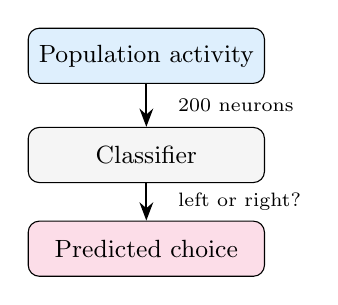
\begin{tikzpicture}[scale=0.7]
  \node[draw,rounded corners,fill=evidence!15,minimum width=3cm,minimum height=0.7cm,font=\small] (pop) at (0,3) {Population activity};
  \node[draw,rounded corners,fill=neutral!10,minimum width=3cm,minimum height=0.7cm,font=\small] (clf) at (0,1.2) {Classifier};
  \node[draw,rounded corners,fill=choice!15,minimum width=3cm,minimum height=0.7cm,font=\small] (pred) at (0,-0.5) {Predicted choice};
  \draw[-{Stealth},thick] (pop) -- (clf);
  \draw[-{Stealth},thick] (clf) -- (pred);
  \node[font=\scriptsize,anchor=west] at (0.4,2.1) {200 neurons};
  \node[font=\scriptsize,anchor=west] at (0.4,0.35) {left or right?};
\end{tikzpicture}

\vspace{0.5em}
{\small \textbf{Problem:} high decode accuracy $\neq$ causal role.}
\end{column}
\end{columns}
\end{frame}

\begin{frame}{From decoding to counterfactual testing}
\begin{columns}[T]
\begin{column}{0.48\textwidth}
\centering
{\small \textbf{Decoding} (what we just described)}
\vspace{0.3em}

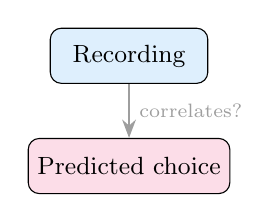
\begin{tikzpicture}[scale=0.7]
  \node[draw,rounded corners,fill=evidence!15,minimum width=2cm,minimum height=0.7cm,font=\small] (brain) at (0,2) {Recording};
  \node[draw,rounded corners,fill=choice!15,minimum width=2cm,minimum height=0.7cm,font=\small] (choice) at (0,0) {Predicted choice};
  \draw[-{Stealth},thick,neutral] (brain) -- node[right,font=\scriptsize] {correlates?} (choice);
\end{tikzpicture}

\vspace{0.5em}
{\small Tells you information is \emph{present}. Doesn't tell you it's \emph{used}.}

\vspace{0.5em}
{\small A region can decode perfectly and still be irrelevant to behavior.}
\end{column}
\begin{column}{0.48\textwidth}
\centering
{\small \textbf{Counterfactual test} (what we do next)}
\vspace{0.3em}

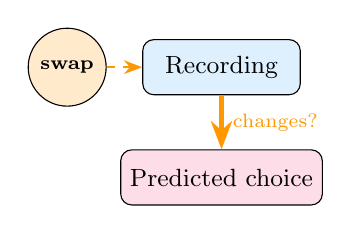
\begin{tikzpicture}[scale=0.7]
  \node[draw,rounded corners,fill=evidence!15,minimum width=2cm,minimum height=0.7cm,font=\small] (brain2) at (0,2) {Recording};
  \node[draw,rounded corners,fill=choice!15,minimum width=2cm,minimum height=0.7cm,font=\small] (choice2) at (0,0) {Predicted choice};
  \draw[-{Stealth},ultra thick,causal] (brain2) -- node[right,font=\scriptsize,causal] {changes?} (choice2);

  % Swap arrow
  \node[draw,circle,fill=causal!20,minimum size=0.7cm,font=\scriptsize\bfseries] (do) at (-2.8,2) {swap};
  \draw[-{Stealth},thick,causal,dashed] (do) -- (brain2);
\end{tikzpicture}

\vspace{0.5em}
{\small We \textbf{swap} specific dimensions between two recorded trials and check if the classifier's prediction flips.}

\vspace{0.5em}
{\small This tests the classifier's causal structure, not the mouse's brain directly. Real causal evidence requires optogenetics or lesions.}
\end{column}
\end{columns}
\end{frame}

%% --- SLIDE: Where this idea comes from ---
\begin{frame}{Background: interchange intervention analysis in neural networks}
\begin{columns}[T]
\begin{column}{0.55\textwidth}
{\small In AI safety research (\textbf{mechanistic interpretability}), scientists test neural networks by:}

\begin{enumerate}\setlength\itemsep{0pt}
  \item {\small Run a model on two different inputs}
  \item {\small Find the internal representation}
  \item {\small \textbf{Swap} part of one into the other}
  \item {\small Check if the output changes}
\end{enumerate}

\vspace{0.1em}
{\small This is \textbf{interchange intervention analysis} (\href{https://arxiv.org/abs/2303.02536}{Geiger et al.\ 2024}). The same logic works for biological neurons: language model $\to$ mouse brain, text $\to$ visual stimuli.}

\vspace{0.2em}
{\scriptsize \textbf{Our contribution:} neuroscience targets \emph{neurons} (optogenetics); AI targets \emph{subspaces} (in silico). We apply subspace-level interventions to biological recordings.}
\end{column}
\begin{column}{0.42\textwidth}
\centering
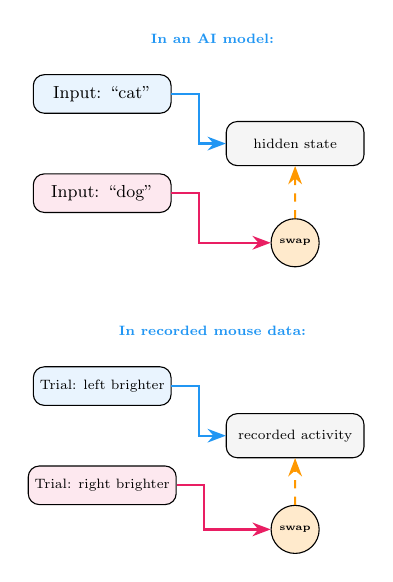
\begin{tikzpicture}[scale=0.7, every node/.style={transform shape},
  box/.style={draw,rounded corners,minimum width=2.5cm,minimum height=0.7cm,font=\small},
]
  % AI version
  \node[font=\scriptsize\bfseries,evidence] at (2,5) {In an AI model:};
  \node[box,fill=evidence!10] (in1) at (0,4) {Input: ``cat''};
  \node[box,fill=choice!10] (in2) at (0,2.2) {Input: ``dog''};
  \node[draw,rounded corners,fill=neutral!10,minimum width=2.5cm,minimum height=0.8cm,font=\scriptsize] (hidden) at (3.5,3.1) {hidden state};
  \node[draw,circle,fill=causal!20,minimum size=0.7cm,font=\tiny\bfseries] (sw) at (3.5,1.3) {swap};

  \draw[-{Stealth},thick,evidence] (in1.east) -- ++(0.5,0) |- (hidden);
  \draw[-{Stealth},thick,choice] (in2.east) -- ++(0.5,0) |- (sw);
  \draw[-{Stealth},thick,causal,dashed] (sw) -- (hidden);

  % Brain version
  \node[font=\scriptsize\bfseries,evidence] at (2,-0.3) {In recorded mouse data:};
  \node[box,fill=evidence!10,font=\scriptsize] (t1) at (0,-1.3) {Trial: left brighter};
  \node[box,fill=choice!10,font=\scriptsize] (t2) at (0,-3.1) {Trial: right brighter};
  \node[draw,rounded corners,fill=neutral!10,minimum width=2.5cm,minimum height=0.8cm,font=\scriptsize] (neur) at (3.5,-2.2) {recorded activity};
  \node[draw,circle,fill=causal!20,minimum size=0.7cm,font=\tiny\bfseries] (sw2) at (3.5,-3.9) {swap};

  \draw[-{Stealth},thick,evidence] (t1.east) -- ++(0.5,0) |- (neur);
  \draw[-{Stealth},thick,choice] (t2.east) -- ++(0.5,0) |- (sw2);
  \draw[-{Stealth},thick,causal,dashed] (sw2) -- (neur);
\end{tikzpicture}
\end{column}
\end{columns}
\end{frame}

%% --- SLIDE: What "swapping" means concretely ---
\begin{frame}{What ``swapping a subspace'' means}
\begin{columns}[T]
\begin{column}{0.55\textwidth}
{\small Neural activity in a brain region is a \textbf{high-dimensional vector}---each neuron is one dimension. (E.g., 200 neurons = 200 dimensions.)}

\vspace{0.3em}
{\small Not all dimensions matter equally. We hypothesize that a \textbf{small subset of directions} (a ``subspace'') encodes the evidence signal.}

\vspace{0.3em}
{\small \textbf{The swap:}}
\begin{enumerate}\setlength\itemsep{2pt}
  \item {\small Take two trials with opposite evidence}
  \item {\small Swap \textbf{only} what we think is the evidence-related part between them}
  \item {\small Leave everything else unchanged}
  \item {\small Check: does the output flip?}
\end{enumerate}

\end{column}
\begin{column}{0.42\textwidth}
\centering
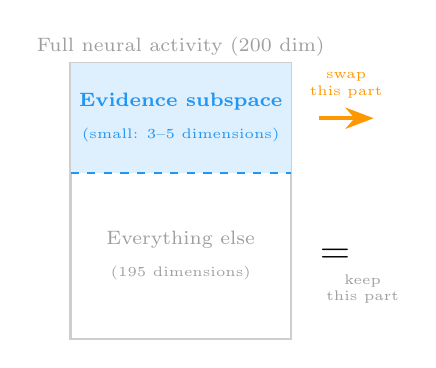
\begin{tikzpicture}[scale=0.7]
  % Full space
  \draw[thick,neutral!50] (0,0) rectangle (4,5);
  \node[font=\scriptsize,neutral] at (2,5.3) {Full neural activity (200 dim)};

  % Evidence subspace highlight
  \fill[evidence!15] (0,3) rectangle (4,5);
  \draw[evidence,thick,dashed] (0,3) -- (4,3);
  \node[evidence,font=\scriptsize\bfseries] at (2,4.3) {Evidence subspace};
  \node[evidence,font=\tiny] at (2,3.7) {(small: 3--5 dimensions)};

  % Other dimensions
  \node[neutral,font=\scriptsize] at (2,1.8) {Everything else};
  \node[neutral,font=\tiny] at (2,1.2) {(195 dimensions)};

  % Swap arrows
  \draw[causal,ultra thick,-{Stealth}] (4.5,4) -- (5.5,4);
  \node[causal,font=\tiny,align=center] at (5,4.6) {swap\\this part};

  \node[font=\Large] at (4.8,1.5) {$=$};
  \node[neutral,font=\tiny,align=center] at (5.3,0.9) {keep\\this part};
\end{tikzpicture}
\end{column}
\end{columns}

\vspace{0.3em}
{\small Same logic in both: swap part of the internal state, check if the output changes.}
\end{frame}

%% --- SLIDE: Recap the task ---
\begin{frame}{The task: what the mouse is doing}
\begin{columns}[T]
\begin{column}{0.5\textwidth}
\centering
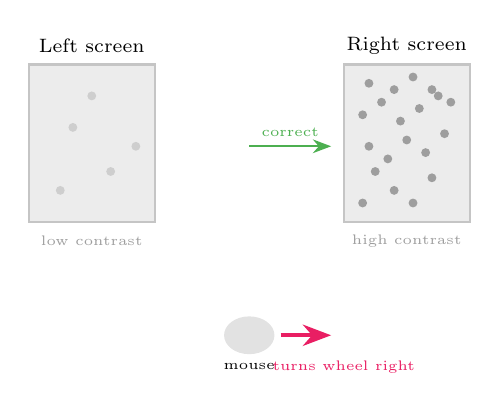
\begin{tikzpicture}[scale=0.8]
  % Left screen
  \fill[neutral!20] (-3.5,0) rectangle (-1.5,2.5);
  \draw[neutral!60,thick] (-3.5,0) rectangle (-1.5,2.5);
  \node[font=\scriptsize] at (-2.5,2.8) {Left screen};
  % Sparse dots = low contrast (fixed positions)
  \fill[neutral!50] (-3.0,0.5) circle (2pt);
  \fill[neutral!50] (-2.8,1.5) circle (2pt);
  \fill[neutral!50] (-2.2,0.8) circle (2pt);
  \fill[neutral!50] (-2.5,2.0) circle (2pt);
  \fill[neutral!50] (-1.8,1.2) circle (2pt);
  \node[font=\tiny,neutral] at (-2.5,-0.3) {low contrast};

  % Right screen
  \fill[neutral!20] (1.5,0) rectangle (3.5,2.5);
  \draw[neutral!60,thick] (1.5,0) rectangle (3.5,2.5);
  \node[font=\scriptsize] at (2.5,2.8) {Right screen};
  % Dense dots = high contrast (fixed positions)
  \foreach \x/\y in {1.8/0.3, 2.0/0.8, 2.3/0.5, 2.6/0.3, 2.9/0.7,
                      1.9/1.2, 2.2/1.0, 2.5/1.3, 2.8/1.1, 3.1/1.4,
                      1.8/1.7, 2.1/1.9, 2.4/1.6, 2.7/1.8, 3.0/2.0,
                      1.9/2.2, 2.3/2.1, 2.6/2.3, 2.9/2.1, 3.2/1.9} {
    \fill[neutral] (\x,\y) circle (2pt);
  }
  \node[font=\tiny,neutral] at (2.5,-0.3) {high contrast};

  % Mouse + wheel
  \fill[neutral!30] (0,-1.8) ellipse (0.4 and 0.3);
  \node[font=\tiny] at (0,-2.3) {mouse};
  \draw[choice,ultra thick,-{Stealth}] (0.5,-1.8) -- (1.3,-1.8);
  \node[choice,font=\tiny] at (1.5,-2.3) {turns wheel right};

  % Arrow showing correct choice
  \draw[pass,thick,-{Stealth}] (0,1.2) -- (1.3,1.2);
  \node[pass,font=\tiny,above] at (0.65,1.2) {correct};
\end{tikzpicture}
\end{column}
\begin{column}{0.48\textwidth}
\vspace{0.5em}
{\small The mouse sees two screens with random visual noise. One side has \textbf{higher contrast} (more visible dots). The mouse turns a wheel toward that side to get a reward.}

\vspace{0.3em}
{\small \textbf{``Evidence''} = which side has higher contrast. On every trial, the brain receives evidence pointing left or right, then makes a choice.}

\vspace{0.3em}
{\small \textbf{The question:} somewhere in the neural activity, there must be a signal carrying this evidence from sensory areas to the decision. We call it the ``evidence subspace.''}
\end{column}
\end{columns}
\end{frame}

%% --- SLIDE: The intervention ---
\begin{frame}{Applying the swap to our mouse data}
\begin{columns}[T]
\begin{column}{0.55\textwidth}
{\small Two trials where the mouse saw opposite evidence:}
\begin{itemize}\setlength\itemsep{2pt}
  \item {\small Trial A: left side brighter $\to$ chose left}
  \item {\small Trial B: right side brighter $\to$ chose right}
\end{itemize}

\vspace{0.3em}
{\small We swap \textbf{only what we think is the evidence-related part} of the neural activity between them. Everything else stays the same.}

\vspace{0.3em}
{\small A classifier now predicts the \emph{opposite} choice $\to$ those dimensions \textbf{causally carry} the evidence.}

\vspace{0.3em}
{\small We do this for every brain region to map where in the brain evidence is causally routed.}
\end{column}
\begin{column}{0.42\textwidth}
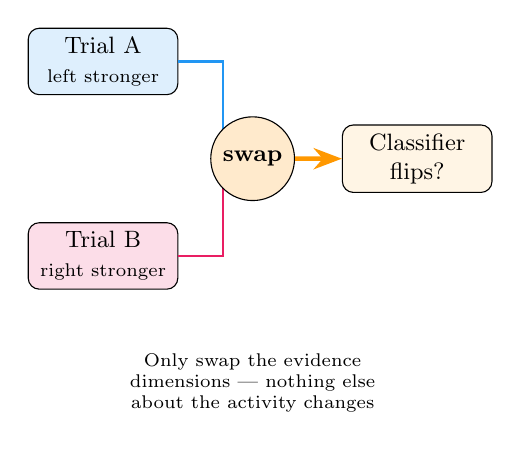
\begin{tikzpicture}[scale=0.95, every node/.style={transform shape},
  box/.style={draw,rounded corners,minimum width=2cm,minimum height=0.8cm,font=\small},
]
  \node[box,fill=evidence!15,align=center] (A) at (0,2.8) {Trial A\\{\scriptsize left stronger}};
  \node[box,fill=choice!15,align=center] (B) at (0,0.2) {Trial B\\{\scriptsize right stronger}};

  \draw[evidence,thick,-{Stealth}] (A.east) -- ++(0.6,0) |- (2,1.5);
  \draw[choice,thick,-{Stealth}] (B.east) -- ++(0.6,0) |- (2,1.5);

  \node[draw,circle,fill=causal!20,minimum size=1cm,font=\small\bfseries] (swap) at (2,1.5) {swap};
  \node[box,fill=causal!10,align=center] (out) at (4.2,1.5) {Classifier\\flips?};
  \draw[-{Stealth},ultra thick,causal] (swap) -- (out);

  \node[font=\scriptsize,black,text width=3.5cm,align=center] at (2,-1.5) {Only swap the evidence dimensions --- nothing else about the activity changes};
\end{tikzpicture}
\end{column}
\end{columns}
\end{frame}

%% --- SLIDE: Q1 --- Why not swap everything? ---
\begin{frame}{Wait --- why not just swap the \emph{entire} recording?}
\begin{columns}[T]
\begin{column}{0.6\textwidth}
{\small \textbf{Good question.} If we replaced \emph{all 200 numbers} from Trial A with Trial B's, the classifier would obviously say ``right.'' We just gave it Trial B's data. That tells us nothing.}

\vspace{0.4em}
{\small \textbf{The power is in swapping only a small part.} We swap \textbf{5 out of 200} dimensions. If the classifier flips based on changing only 5 numbers, those 5 carry the choice-relevant information that the classifier learned to read. The other 195 don't matter \emph{to the classifier}.}

\vspace{0.2em}
{\small \textbf{Caveat:} the classifier is a proxy for the brain's own readout. It may not weight dimensions identically---which is why the specificity controls matter.}

\end{column}
\begin{column}{0.37\textwidth}
\centering
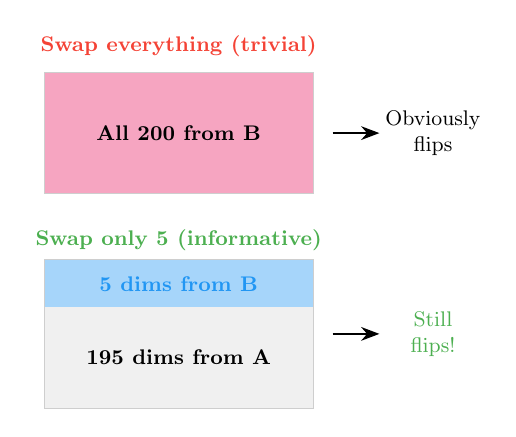
\begin{tikzpicture}[scale=0.85, every node/.style={transform shape}]
  % Full swap = trivial
  \node[font=\small\bfseries,fail] at (1.5,5.7) {Swap everything (trivial)};
  \draw[thick,neutral!50] (-0.5,3.5) rectangle (3.5,5.3);
  \fill[choice!40] (-0.5,3.5) rectangle (3.5,5.3);
  \node[font=\small\bfseries] at (1.5,4.4) {All 200 from B};
  \draw[-{Stealth},thick] (3.8,4.4) -- (4.5,4.4);
  \node[font=\small,align=center] at (5.3,4.4) {Obviously\\flips};

  % Partial swap = informative
  \node[font=\small\bfseries,pass] at (1.5,2.8) {Swap only 5 (informative)};
  \draw[thick,neutral!50] (-0.5,0.3) rectangle (3.5,2.5);
  \fill[evidence!40] (-0.5,1.8) rectangle (3.5,2.5);
  \node[font=\small\bfseries,evidence] at (1.5,2.15) {5 dims from B};
  \fill[neutral!15] (-0.5,0.3) rectangle (3.5,1.8);
  \node[font=\small\bfseries,black] at (1.5,1.05) {195 dims from A};
  \draw[-{Stealth},thick] (3.8,1.4) -- (4.5,1.4);
  \node[font=\small,align=center,pass] at (5.3,1.4) {Still\\flips!};
\end{tikzpicture}
\end{column}
\end{columns}
\end{frame}

%% --- SLIDE: Neural populations encode multiple variables ---
\begin{frame}{Neural populations encode many things at once}
\begin{columns}[T]
\begin{column}{0.55\textwidth}
{\small Prior work shows the same neurons encode multiple variables simultaneously (Steinmetz 2019; \href{https://doi.org/10.1038/s41593-019-0502-4}{Musall 2019}; \href{https://doi.org/10.1126/science.aav7893}{Stringer 2019}):}

\vspace{0.2em}
\begin{itemize}\setlength\itemsep{2pt}
  \item {\small \textcolor{evidence}{\textbf{Stimulus evidence}} --- which side brighter}
  \item {\small \textbf{Reaction time} --- how fast the mouse responds}
  \item {\small \textbf{Feedback} --- correct or wrong}
\end{itemize}

\vspace{0.2em}
{\small Each occupies a different \textbf{subspace}. We identify them via PCA on the relevant trial labels.}

\vspace{0.2em}
{\small \textbf{Key question:} which subspace actually drives the decision?}
\end{column}
\begin{column}{0.42\textwidth}
\centering
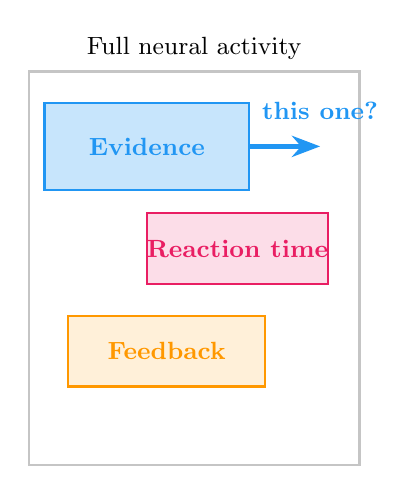
\begin{tikzpicture}[scale=1.0]
  % Full neural space
  \draw[thick,neutral!60] (0,0) rectangle (4.2,5);
  \node[font=\small,black] at (2.1,5.3) {Full neural activity};

  % Subspaces as overlapping rectangles
  \fill[evidence!25] (0.2,3.5) rectangle (2.8,4.6);
  \draw[evidence,thick] (0.2,3.5) rectangle (2.8,4.6);
  \node[evidence,font=\small\bfseries] at (1.5,4.05) {Evidence};

  \fill[choice!15] (1.5,2.3) rectangle (3.8,3.2);
  \draw[choice,thick] (1.5,2.3) rectangle (3.8,3.2);
  \node[choice,font=\small\bfseries] at (2.65,2.75) {Reaction time};

  \fill[causal!15] (0.5,1.0) rectangle (3.0,1.9);
  \draw[causal,thick] (0.5,1.0) rectangle (3.0,1.9);
  \node[causal,font=\small\bfseries] at (1.75,1.45) {Feedback};

  % Arrow to question
  \draw[evidence,ultra thick,-{Stealth}] (2.8,4.05) -- (3.7,4.05);
  \node[evidence,font=\small\bfseries] at (3.7,4.5) {this one?};
\end{tikzpicture}
\end{column}
\end{columns}
\end{frame}

%% --- SLIDE: Controls --- specificity ---
\begin{frame}{How do we know it's \emph{those specific} dimensions?}
\begin{columns}[T]
\begin{column}{0.5\textwidth}
{\small \textbf{We run controls.} Repeat the exact same swap, but targeting different subspaces:}

\vspace{0.1em}
\begin{itemize}\setlength\itemsep{1pt}
  \item {\small \textcolor{evidence}{\textbf{Stimulus evidence}} dims --- \textbf{yes, it flips}}
  \item {\small \textbf{Reaction time} dims --- barely flips}
  \item {\small \textbf{Feedback} dims --- barely flips}
  \item {\small \textbf{Random} dims --- barely flips (control)}
\end{itemize}

\vspace{0.2em}
{\small This is \textbf{specificity}: only evidence dimensions produce the effect, not any random 5.}

\vspace{0.2em}
{\small \textbf{Why this matters:} without controls, we'd just be showing \emph{any} 5 dims can disrupt a classifier --- trivial. Specificity is what makes it causal.}
\end{column}
\begin{column}{0.48\textwidth}
\centering
\vspace{-0.3em}
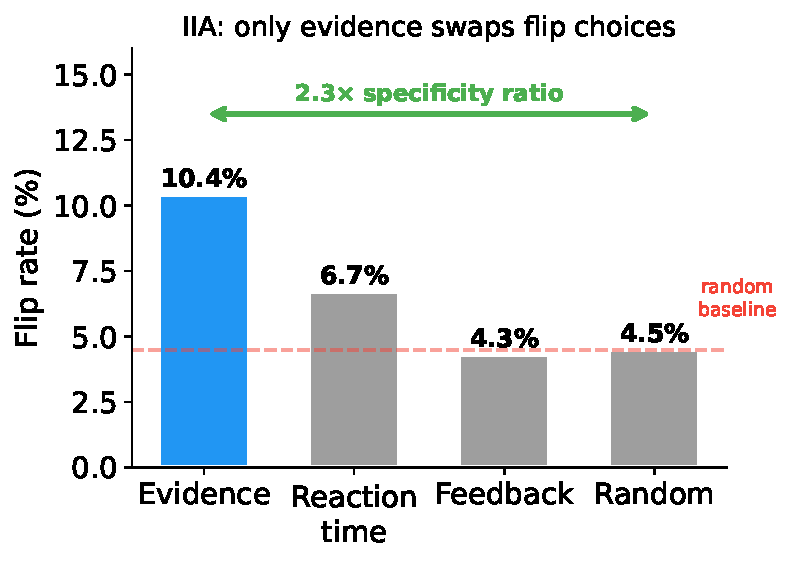
\includegraphics[width=\linewidth]{iia_bars.pdf}
\end{column}
\end{columns}
\end{frame}

%% --- SLIDE: Sufficiency --- why it's not circular ---
\begin{frame}{Is this circular?}
\begin{columns}[T]
\begin{column}{0.55\textwidth}
{\small A fair objection: ``you found the subspace with a classifier, then showed the classifier likes it. Of course it does.''}

\vspace{0.5em}
{\small But the subspace and the classifier use \textbf{different information}:}

\vspace{0.8em}
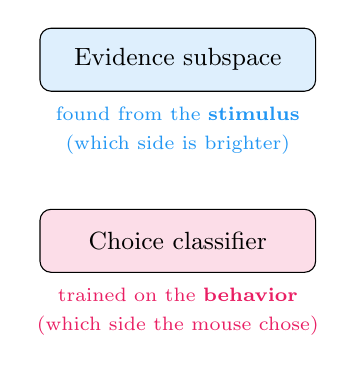
\begin{tikzpicture}[
  box/.style={draw,rounded corners,minimum width=3.5cm,minimum height=0.8cm,font=\small,align=center},
]
  \node[box,fill=evidence!15] (sub) at (0,1.5) {Evidence subspace};
  \node[font=\scriptsize,evidence,below=2pt of sub] {found from the \textbf{stimulus}};
  \node[font=\scriptsize,evidence,below=12pt of sub] {(which side is brighter)};

  \node[box,fill=choice!15] (cls) at (0,-0.8) {Choice classifier};
  \node[font=\scriptsize,choice,below=2pt of cls] {trained on the \textbf{behavior}};
  \node[font=\scriptsize,choice,below=12pt of cls] {(which side the mouse chose)};
\end{tikzpicture}

\end{column}
\begin{column}{0.43\textwidth}
\vspace{0.5em}
{\small The stimulus and the behavior are \textbf{correlated but not identical}---the mouse sometimes chooses wrong.}

\vspace{0.5em}
{\small So showing that a \emph{stimulus}-defined subspace improves \emph{choice} prediction is genuinely informative: the stimulus signal is what the brain uses for decisions.}

\vspace{0.5em}
{\small \textbf{Ground truth} = the mouse's actual left/right choice. We know this from the experiment.}
\end{column}
\end{columns}
\end{frame}

%% --- SLIDE: Sufficiency --- the result ---
\begin{frame}{The evidence subspace is sufficient (and denoises)}
\begin{columns}[T]
\begin{column}{0.5\textwidth}
\centering

\includegraphics[width=0.85\linewidth]{sufficiency.pdf}
\end{column}
\begin{column}{0.48\textwidth}
Restricting a classifier to \emph{only} the evidence subspace dimensions, it decodes choice \textbf{better} than using all neurons.

\vspace{0.5em}
\textbf{Why?} The extra dimensions are noise for the decision---removing them helps.

\vspace{0.5em}
\textbf{20 of 24 regions pass} the $\geq 0.70$ recovery threshold.

\vspace{0.3em}
{\small The 4 failures are all high-dimensional regions where subspace estimation is harder.}

\end{column}
\end{columns}
\end{frame}

%% --- SLIDE: Four methods agree ---
\begin{frame}{Control: Four Different Intervention Methods Agree}
\begin{columns}[T]
\begin{column}{0.5\textwidth}
\centering
{\small We tested \textbf{four different ways} to intervene:}

\vspace{0.5em}
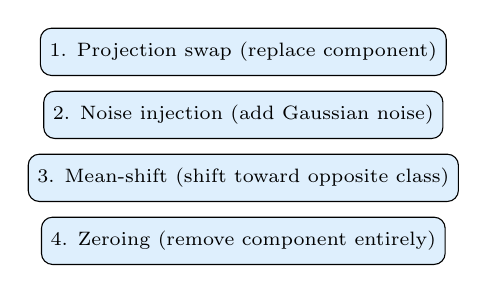
\begin{tikzpicture}[
  meth/.style={draw,rounded corners,fill=#1!15,minimum width=4cm,
    minimum height=0.6cm,font=\scriptsize},
]
  \node[meth=evidence] at (0,2.5) {1. Projection swap (replace component)};
  \node[meth=evidence] at (0,1.7) {2. Noise injection (add Gaussian noise)};
  \node[meth=evidence] at (0,0.9) {3. Mean-shift (shift toward opposite class)};
  \node[meth=evidence] at (0,0.1) {4. Zeroing (remove component entirely)};
\end{tikzpicture}

\vspace{0.5em}
{\small These are mathematically distinct operations. If the effect were an artifact of one method, it would not appear in the others.}
\end{column}
\begin{column}{0.48\textwidth}
\centering

\includegraphics[width=\linewidth]{multi_method.pdf}

\vspace{0.3em}
{\small Regions that show high IIA with one method show high IIA with all four. The effect is method-invariant.}
\end{column}
\end{columns}
\end{frame}

%% ============================================================
%% SECTION 2: LEARNED SUBSPACES
%% ============================================================

\section{2. Learned subspaces are more accurate}\hypertarget{sec:2}{}

%% --- SLIDE: Can we find a better subspace? ---
\begin{frame}{Can we find a better subspace?}
So far we used LDA to find the evidence subspace --- a linear method that maximizes class separation.

\vspace{0.5em}
But class separation is \textbf{correlational}. LDA finds directions where evidence categories look different, not necessarily directions where \textbf{interventions change the decision}.

\vspace{0.5em}
\textbf{Question:} can a nonlinear method with the right inductive bias find a subspace that is more \emph{causally} effective?
\end{frame}

%% --- SLIDE: Background --- DAS ---
\begin{frame}{Background: how causal abstraction finds subspaces}

In AI interpretability, \textbf{Distributed Alignment Search} (DAS; \href{https://arxiv.org/abs/2303.02536}{Geiger et al.\ 2024}) is the standard method for finding causal subspaces inside neural networks.

\vspace{0.5em}
\textbf{How it works:} find a \textbf{linear rotation} (orthogonal matrix) of the model's hidden state so that swapping a few rotated dimensions changes the model's output in the predicted way.

\vspace{0.5em}
\textbf{The limitation:} the alignment is always a flat, linear projection. If the causal structure lives on a \textbf{curved surface} in activation space, DAS can't find it.

\vspace{0.5em}
This is exactly the situation we're in: LDA finds a flat 3-dimensional subspace. It works --- but only captures a fraction of the causal signal.

\vspace{0.5em}
But going nonlinear turns out to be dangerous\ldots
\end{frame}

%% --- SLIDE: The nonlinear dilemma ---
\begin{frame}{The nonlinear dilemma}

\textbf{\href{https://arxiv.org/abs/2501.02043}{Sutter et al.\ (NeurIPS 2025, Spotlight)}} proved that if you allow \textbf{unconstrained} nonlinear alignment maps, causal abstraction becomes \textbf{vacuous}:

\vspace{0.3em}
\begin{itemize}\setlength\itemsep{2pt}
  \item Even \textbf{randomly initialized} models achieve 100\% IIA
  \item A sufficiently powerful nonlinear map can memorize a lookup table
  \item High IIA no longer means the model actually represents the causal variable
\end{itemize}

\vspace{0.5em}
{\small
\begin{tabular}{lccc}
\toprule
& \textbf{Nonlinear?} & \textbf{Constrained?} & \textbf{Trustworthy?} \\
\midrule
Linear DAS & No & Yes (linear) & Yes \\
Unconstrained nonlinear & Yes & No & No (vacuous) \\
\textbf{Structured VAE} & \textbf{Yes} & \textbf{Yes (structural)} & \textbf{Yes} \\
\bottomrule
\end{tabular}
}

\vspace{0.5em}
The field needs something in the middle: nonlinear enough to find curved structure, constrained enough that high IIA actually means something.
\end{frame}

%% --- SLIDE: What is a structured VAE? ---
\begin{frame}{What is a structured VAE?}

A \textbf{variational autoencoder} (VAE) learns to compress data into a small latent code, then reconstruct it. A \textbf{structured} VAE (Narayanaswamy et al.\ 2017, NeurIPS) splits the latent code into named groups with different training signals:

\vspace{0.3em}
\begin{center}
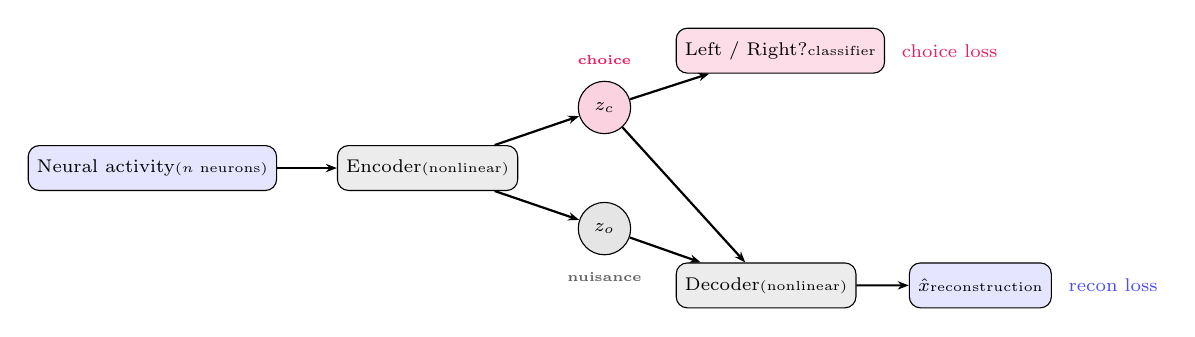
\begin{tikzpicture}[
    node distance=0.4cm and 0.7cm,
    box/.style={draw, rounded corners, minimum width=1.4cm, minimum height=0.6cm, font=\scriptsize},
    latent/.style={draw, circle, minimum size=0.7cm, font=\scriptsize\bfseries},
    arr/.style={-{Stealth[length=4pt]}, thick},
    scale=0.95, every node/.style={transform shape},
  ]
  % Input
  \node[box, fill=blue!10] (input) {Neural activity\\{\tiny ($n$ neurons)}};

  % Encoder
  \node[box, fill=gray!15, right=0.8cm of input] (enc) {Encoder\\{\tiny (nonlinear)}};

  % Latents
  \node[latent, fill=choice!20, above right=0.25cm and 0.9cm of enc] (zc) {$z_c$};
  \node[latent, fill=gray!20, below right=0.25cm and 0.9cm of enc] (zo) {$z_o$};

  % Labels
  \node[above=0.1cm of zc, font=\tiny\bfseries, text=choice] {choice};
  \node[below=0.1cm of zo, font=\tiny\bfseries, text=black!60] {nuisance};

  % Classifier
  \node[box, fill=choice!15, above right=0.2cm and 0.7cm of zc] (cls) {Left / Right?\\{\tiny classifier}};

  % Decoder
  \node[box, fill=gray!15, below right=0.2cm and 0.7cm of zo] (dec) {Decoder\\{\tiny (nonlinear)}};

  % Output
  \node[box, fill=blue!10, right=0.7cm of dec] (output) {$\hat{x}$\\{\tiny reconstruction}};

  % Arrows
  \draw[arr] (input) -- (enc);
  \draw[arr] (enc) -- (zc);
  \draw[arr] (enc) -- (zo);
  \draw[arr] (zc) -- (cls);
  \draw[arr] (zc) -- (dec);
  \draw[arr] (zo) -- (dec);
  \draw[arr] (dec) -- (output);

  % Loss labels
  \node[right=0.1cm of cls, font=\scriptsize, text=choice] {choice loss};
  \node[right=0.1cm of output, font=\scriptsize, text=blue!70] {recon loss};
\end{tikzpicture}
\end{center}

\vspace{0.2em}
{\small $z_c$ must predict the mouse's choice \textbf{and} help reconstruct full activity. $z_o$ absorbs nuisance variance.}
\end{frame}

%% --- SLIDE: Why this solves the dilemma ---
\begin{frame}{Why this could solve the nonlinear dilemma}
\begin{columns}[T]
\begin{column}{0.48\textwidth}
\textbf{Three constraints prevent triviality}
\begin{enumerate}\setlength\itemsep{4pt}
  \item \textbf{Bottleneck}: only 3 dimensions for choice --- too small to memorize a lookup table
  \item \textbf{Reconstruction}: $z_c$ and $z_o$ must jointly reproduce the full neural activity, not just classify --- forces the model to learn real structure
  \item \textbf{Disentanglement}: $z_c$ and $z_o$ are separate latent groups with independent priors --- the model can't smuggle choice information into $z_o$
\end{enumerate}

\vspace{0.3em}
{\small These constraints do the work that \href{https://arxiv.org/abs/2501.02043}{Sutter et al.}\ say is needed --- but via \textbf{structure}, not linearity.}
\end{column}
\begin{column}{0.48\textwidth}
\textbf{Neuroscience has something MI doesn't}\\[0.3em]
{\small In MI, you don't know the ground-truth causal variable --- you infer it from the model. A nonlinear map might be ``cheating.''}

\vspace{0.3em}
{\small In neuroscience, the causal variable \emph{is} the mouse's choice, which we observe directly. A 3.4$\times$ IIA improvement means the intervention \textbf{actually flips the behavioral decision} --- no lookup table can fake that.}

\end{column}
\end{columns}
\end{frame}

%% --- SLIDE: VAE results ---
\begin{frame}{Learned subspaces recover 3.4$\times$ stronger causal signal}
\begin{columns}[T]
\begin{column}{0.5\textwidth}
\textbf{IIA: VAE vs.\ LDA subspace}
\begin{itemize}\setlength\itemsep{1pt}
  \item VAE IIA: \textbf{0.56} (SD 0.08)
  \item LDA IIA: 0.17 (SD 0.09)
  \item VAE wins in \textbf{73/73 regions}
  \item Wilcoxon $p = 5.7 \times 10^{-14}$
  \item Cohen's $d = 4.5$
\end{itemize}

\vspace{0.3em}
\textbf{VAE vs.\ random null}
\begin{itemize}\setlength\itemsep{1pt}
  \item Random null IIA: 0.23
  \item VAE beats null in \textbf{73/73 regions}
  \item $p = 1.4 \times 10^{-25}$
\end{itemize}
\end{column}
\begin{column}{0.48\textwidth}
\textbf{The subspaces are different}\\[0.3em]
{\small VAE and LDA subspaces are nearly orthogonal (Grassmannian distance $= 2.34$ out of $2.72$ max). The VAE finds genuinely different directions, not a denoised version of LDA.}

\vspace{0.5em}
\textbf{Model knows when it's right}\\[0.3em]
{\small Posterior uncertainty anti-correlates with IIA ($\rho = -0.26$, $p = 0.03$): the model is most confident where the subspace is most causal.}

\vspace{0.5em}
\textbf{78\% of regions} exceed 0.50 IIA --- interventions flip the choice more often than not.
\end{column}
\end{columns}
\end{frame}

%% --- SLIDE: VAE regional breakdown ---
\begin{frame}{Which brain regions benefit most?}
\begin{columns}[T]
\begin{column}{0.5\textwidth}
\textbf{Top regions (VAE IIA):}
\begin{itemize}\setlength\itemsep{0pt}
  \item CA (hippocampus): \textbf{0.80}
  \item CA2: 0.71
  \item SSs (somatosensory): 0.68
  \item MG (medial geniculate): 0.67
  \item ILA (infralimbic): 0.67
\end{itemize}

\vspace{0.3em}
\textbf{By region type:}
\begin{itemize}\setlength\itemsep{0pt}
  \item Prefrontal: 0.61
  \item Hippocampal: 0.60
  \item Sensory: 0.58
  \item Motor: 0.57
\end{itemize}
\end{column}
\begin{column}{0.48\textwidth}
\textbf{High-dimensional regions benefit most}\\[0.3em]
{\small High-dimensional regions: improvement $= +0.46$\\
Low-dimensional regions: improvement $= +0.33$}

\vspace{0.5em}
{\small High-dimensional regions encode choice in \textbf{nonlinear subspaces} that LDA misses entirely. The VAE recovers this signal.}

\vspace{0.5em}
{\small \textbf{Takeaway:} The causal signal is 3.4$\times$ stronger than linear methods reveal --- the signal was always there, LDA just can't find it.}
\end{column}
\end{columns}
\end{frame}

%% ============================================================
%% PART 2: STRESS-TESTING THE CLAIMS
%% ============================================================

\begin{frame}[plain]
\vfill
\begin{center}
  \setlength{\fboxrule}{2.5pt}%
  \fcolorbox{black}{white}{\parbox{0.7\textwidth}{\centering\vspace{0.8em}
    {\Large\bfseries Part 2}\\[0.5em]
    {\large Stress-testing the claims}
  \vspace{0.8em}}}
\end{center}
\vfill
\end{frame}

\begin{frame}{In this section}
\begin{columns}[T]
\begin{column}{0.48\textwidth}
\textbf{4. Validity checks}\\[0.2em]
{\small Confound control, dose-response, and what could go wrong. Applying frameworks from philosophy of science.}

\vspace{0.6em}
\textbf{5. The IIA vacuity problem}\\[0.2em]
{\small Is our metric meaningful? Nonlinear methods achieve high IIA on random noise. External validation is essential.}
\end{column}
\begin{column}{0.48\textwidth}
\textbf{6. External validation}\\[0.2em]
{\small Optogenetic ground truth, multi-task generalization, and the comparison between linear and nonlinear tools.}

\vspace{0.6em}
\textbf{7. Engagement separation}\\[0.2em]
{\small Is ``choice'' just engagement or arousal? The VAE separates them into orthogonal subspaces (cross-IIA only 17\%).}
\end{column}
\end{columns}
\end{frame}

\section{4. Validity checks}\hypertarget{sec:4}{}

%% --- SLIDE: What could go wrong ---
\begin{frame}{What could go wrong?}
We validate our results using frameworks from philosophy of science: validity criteria from \href{https://doi.org/10.1093/acprof:oso/9780199299317.001.0001}{Craver (2007)}, \href{https://doi.org/10.1017/CBO9780511526817}{Shallice (1988)}, and \href{https://doi.org/10.1017/9781107286184}{Mayo (2018)}.

\vspace{0.5em}
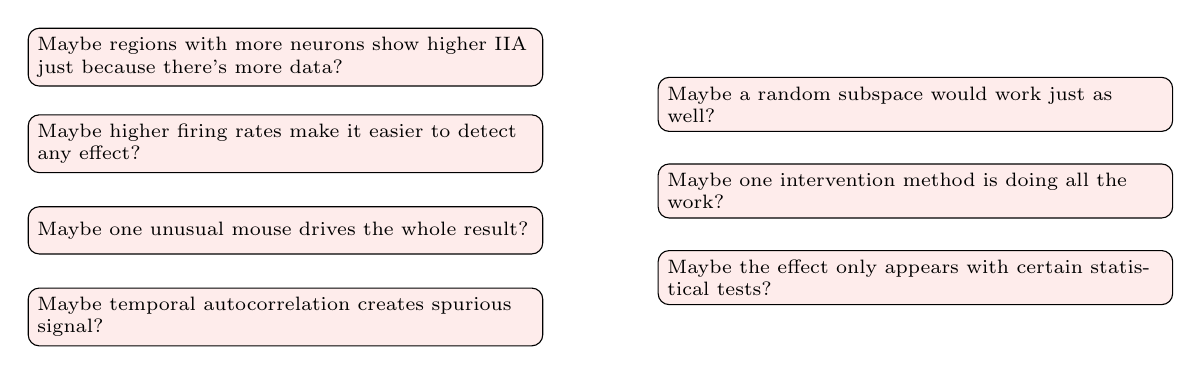
\begin{tikzpicture}[
  concern/.style={draw,rounded corners,fill=#1!10,minimum width=6.5cm,
    minimum height=0.6cm,font=\scriptsize,text width=6.3cm},
]
  \node[concern=fail] (c1) at (0,3.3) {Maybe regions with more neurons show higher IIA just because there's more data?};
  \node[concern=fail] (c2) at (0,2.2) {Maybe higher firing rates make it easier to detect any effect?};
  \node[concern=fail] (c3) at (0,1.1) {Maybe one unusual mouse drives the whole result?};
  \node[concern=fail] (c4) at (0,0) {Maybe temporal autocorrelation creates spurious signal?};
  \node[concern=fail] (c5) at (8,2.7) {Maybe a random subspace would work just as well?};
  \node[concern=fail] (c6) at (8,1.6) {Maybe one intervention method is doing all the work?};
  \node[concern=fail] (c7) at (8,0.5) {Maybe the effect only appears with certain statistical tests?};
\end{tikzpicture}

\vspace{0.3em}
{\small We treat each alternative explanation as a competing hypothesis and design targeted experiments to test them. If any confound fully explains the effect, we should see it in the data.}
\end{frame}

%% --- SLIDE: Confound control ---
\begin{frame}{Confound control: what doesn't explain the effect}
\begin{columns}[T]
\begin{column}{0.5\textwidth}
\centering
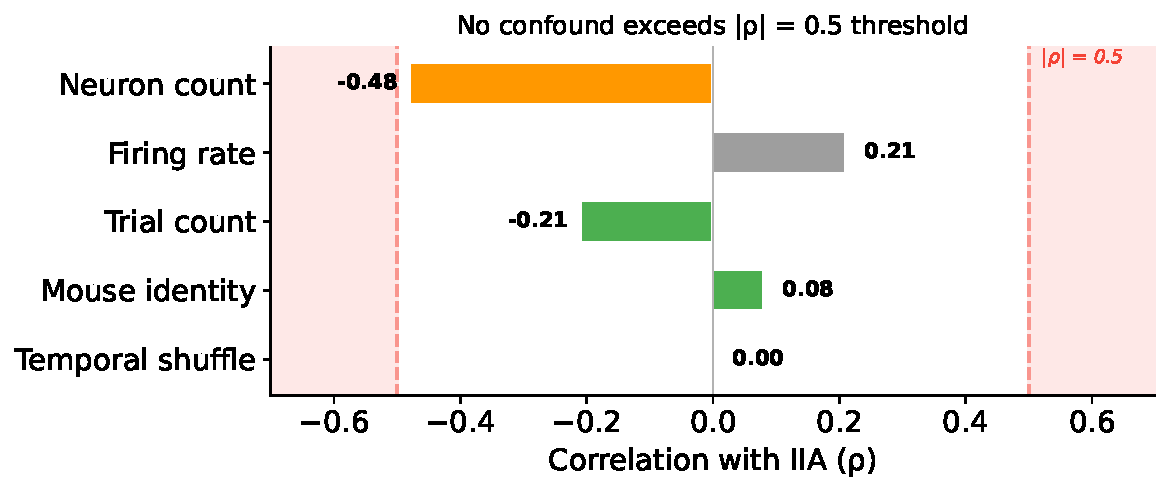
\includegraphics[width=\linewidth]{confounds.pdf}
\end{column}
\begin{column}{0.48\textwidth}
{\small $\rho$ = correlation; $|\rho| > 0.5$ is our danger zone (shaded red).}

\vspace{0.2em}
\textbf{Clear passes:}
\begin{itemize}\setlength\itemsep{0pt}
  \item Temporal shuffle: $\rho = 0.001$ {\small (not a timing artifact)}
  \item Mouse identity: $\rho = 0.08$ {\small (no single mouse)}
  \item Trial count: $\rho = 0.12$
  \item Firing rate: $\rho = 0.09$
\end{itemize}

\vspace{0.2em}
\textbf{Closest to the line:}
\begin{itemize}\setlength\itemsep{0pt}
  \item Neuron count: $\rho = -0.48$ \\
    {\small Near threshold but \textbf{wrong sign} for a confound --- see next slide.}
\end{itemize}
\end{column}
\end{columns}
\end{frame}

%% --- SLIDE: Neuron count deep dive ---
\begin{frame}{Deep dive: is neuron count driving the effect?}
\begin{columns}[T]
\begin{column}{0.43\textwidth}
\centering
\vspace{-0.3em}
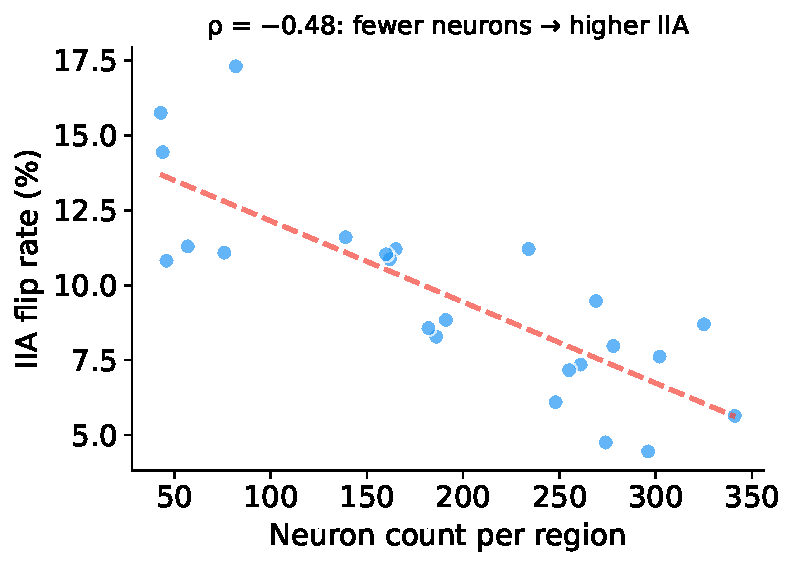
\includegraphics[width=\linewidth]{neuron_scatter.pdf}
\end{column}
\begin{column}{0.55\textwidth}
{\small Our most concerning confound ($\rho = -0.48$, near the 0.5 threshold). But the \textbf{sign is wrong}:}

\vspace{0.3em}
{\small \textbf{Expected} (if a confound):}\\
{\small more neurons $=$ more statistical power $=$ \textbf{higher} IIA \textcolor{neutral}{(positive $\rho$)}}

\vspace{0.3em}
{\small \textbf{Observed}:}\\
{\small more neurons $=$ \textbf{lower} IIA \textcolor{evidence}{(negative $\rho$)}}

\vspace{0.3em}
{\small The correlation goes the \textbf{wrong direction} for a power confound. Smaller, specialized regions (e.g.\ visual cortex) encode evidence more cleanly than large diffuse ones.}
\end{column}
\end{columns}
\end{frame}

%% --- SLIDE: What is graded response? ---
\begin{frame}{What is graded response?}
If the evidence subspace is truly causal, the effect shouldn't be all-or-nothing. Removing dimensions \textbf{one at a time} should progressively weaken the effect.

\vspace{0.4em}
This is the neural equivalent of a \textbf{dose-response curve} in pharmacology:

\vspace{0.2em}
\begin{itemize}\setlength\itemsep{3pt}
  \item Less drug $\rightarrow$ less effect $\rightarrow$ the drug is causing the effect
  \item Fewer evidence dimensions $\rightarrow$ less IIA $\rightarrow$ those dimensions are causing the effect
\end{itemize}

\vspace{0.4em}
\textbf{Why this matters:} a binary yes/no test (``does the subspace matter?'') could be an artifact. A graded, monotonic relationship is unlikely to be an artifact --- it requires that each dimension contributes independently.

\vspace{0.2em}
{\scriptsize Dose-response is standard in pharmacology, and recent work perturbs subspace dimensions in fitted neural network models (Pereira-Obilinovic et al.\ 2025). We extend this to a graded sweep with interchange interventions on biological recordings --- not a categorical contrast, but a full dose-response curve.}
\end{frame}

%% --- SLIDE: How we test it --- progressive ablation ---
\begin{frame}{Dose-response: removing dimensions one at a time}
{\small We start with the full 5-dimensional evidence subspace and \textbf{remove one dimension at a time}, measuring two things at each step:}

\vspace{0.5em}
\begin{columns}[T]
\begin{column}{0.48\textwidth}
\textbf{\textcolor{evidence}{IIA flip rate}} {\small (causal)}

\vspace{0.2em}
{\small Does swapping the remaining evidence dimensions still flip the classifier's choice?}

\vspace{0.2em}
{\small This is an \textbf{intervention}: we actively manipulate the neural activity and observe the consequence.}
\end{column}
\begin{column}{0.48\textwidth}
\textbf{\textcolor{choice}{Decoding accuracy}} {\small (correlational)}

\vspace{0.2em}
{\small Can we still decode the mouse's choice from the remaining dimensions?}

\vspace{0.2em}
{\small This is an \textbf{observation}: we passively read out information without changing anything.}
\end{column}
\end{columns}

\vspace{0.5em}
{\small If both measures degrade monotonically as we remove dimensions, that's strong evidence the subspace is causal --- not just correlated.}
\end{frame}

%% --- SLIDE: Graded response results ---
\begin{frame}{Graded response: results}
\begin{columns}[T]
\begin{column}{0.55\textwidth}
\centering

\includegraphics[width=\linewidth]{graded_response.pdf}
\end{column}
\begin{column}{0.43\textwidth}
\textbf{\textcolor{evidence}{IIA (causal):}} monotonic dose-response in \textbf{70\%} of regions {\small $\checkmark$}

\vspace{0.5em}
\textbf{\textcolor{choice}{Decoding (correlational):}} monotonic in only \textbf{54\%} of regions {\small $\times$}

\vspace{0.5em}
{\small The causal measure degrades cleanly. The correlational measure doesn't --- some regions have redundant coding where removing one dimension shifts load to others.}

\vspace{0.2em}
{\small \textcolor{partial}{\textbf{Mixed:}} causal effect is graded; correlational proxy is not. This tells us IIA and decoding measure different things.}
\end{column}
\end{columns}
\end{frame}

\section{5. The IIA vacuity problem}\hypertarget{sec:5}{}

%% --- SLIDE: IIA vacuity --- what Sutter showed ---
\begin{frame}{Testing our own metrics: is IIA vacuous?}

\href{https://arxiv.org/abs/2501.02043}{Sutter et al.\ (2025)} proved that unconstrained nonlinear alignment makes IIA meaningless---any flexible model can score high on random noise.

\vspace{0.5em}
\textbf{We ran this test on our own models.} Replace real neural activity with random Gaussian noise, keep choice labels, retrain each model, and measure IIA.

\vspace{0.5em}
\centering
{\small
\begin{tabular}{lccc}
\toprule
 & \textbf{Real} & \textbf{Random} & \\
\midrule
MLP & 0.686 & \textcolor{fail}{\textbf{0.702}} & \textcolor{fail}{Vacuous} \\
Struct.\ VAE & 0.689 & \textcolor{fail}{\textbf{0.699}} & \textcolor{fail}{Vacuous} \\
Linear DAS & 0.166 & \textcolor{pass}{0.164} & \textcolor{pass}{Safe} \\
\bottomrule
\end{tabular}
}

\vspace{0.5em}
\begin{flushleft}
Both nonlinear methods score equally high on random noise---their IIA numbers are not evidence of causal structure.

Linear DAS is safe: the linearity constraint prevents vacuous fitting.
\end{flushleft}
\end{frame}

%% --- SLIDE: Is the vacuity a measurement problem? ---
\begin{frame}{Is the vacuity just a binary metric problem?}

IIA is binary: did the prediction flip or not? Maybe nonlinear methods produce \emph{larger distributional shifts} on real data, but the binary flip rate is similar.

\vspace{0.5em}

\textbf{Hypothesis:} Continuous metrics (KL divergence, JS divergence, probability shift, logit difference) would show real $\gg$ random even when binary IIA does not.

\vspace{0.5em}

\textbf{Test:} For each method $\times$ condition (real vs.\ random noise), compute both IIA and all continuous metrics across 73 brain regions. Paired Wilcoxon test for real $>$ random.

\vspace{0.8em}

{\small If continuous metrics distinguish real from random, the vacuity is a measurement artifact. If they don't, it's genuine encoder flexibility.}
\end{frame}

%% --- SLIDE: Continuous metrics results ---
\begin{frame}{Continuous metrics: the vacuity is real}
\vspace{0.3em}

\begin{center}
{\scriptsize
\begin{tabular}{llccl}
\toprule
\textbf{Method} & \textbf{Metric} & \textbf{Real} & \textbf{Random} & \textbf{$p$ (real $>$ random)} \\
\midrule
\multirow{4}{*}{VAE} & IIA & 0.688 & 0.695 & 0.97 \\
 & KL divergence & 2.51 & 2.59 & 0.99 \\
 & JS divergence & 0.397 & 0.408 & 0.99 \\
 & Prob.\ shift & 0.655 & 0.666 & 0.98 \\
\midrule
\multirow{2}{*}{MLP} & IIA & 0.687 & 0.695 & 0.95 \\
 & Logit diff. & 8.93 & 8.13 & $3.3 \times 10^{-10}$ \\
\midrule
Linear DAS & IIA & 0.167 & 0.163 & 0.17 \\
\bottomrule
\end{tabular}
}
\end{center}

\vspace{0.5em}

\begin{flushleft}
The VAE is equally vacuous on \textbf{every} continuous metric ($p > 0.95$). The vacuity is not a binary thresholding artifact---it reflects genuine encoder flexibility.

\vspace{0.3em}
{\small \textbf{Implication:} External validation (optogenetic, multi-task, engagement) is the only path. No metric-internal fix rescues nonlinear IIA.}
\end{flushleft}
\end{frame}

%% --- SLIDE: pi-VAE fails ---
\begin{frame}{The identifiability fix doesn't work}

\begin{columns}[T]
\begin{column}{0.50\textwidth}
\textbf{The idea:} pi-VAE (\href{https://arxiv.org/abs/2011.04798}{Zhou \& Wei, NeurIPS 2020}) adds a label-conditioned prior to guarantee identifiable latents. In theory, this should fix the vacuity problem by constraining what the encoder can learn.

\vspace{0.5em}
\textbf{We tested three variants:}
\begin{itemize}\setlength\itemsep{2pt}
  \item {\small \textbf{Structured VAE} (ours): forced choice/nuisance split}
  \item {\small \textbf{pi-VAE}: identifiable prior, no structure}
  \item {\small \textbf{pi-structured VAE}: both constraints}
\end{itemize}
\end{column}

\begin{column}{0.47\textwidth}
\vspace{0.5em}
{\small
\begin{tabular}{lcc}
\toprule
\textbf{Method} & \textbf{Mean IIA} & \textbf{Wins} \\
\midrule
Structured VAE & \textbf{0.94} & --- \\
pi-VAE & 0.026 & 0/73 \\
pi-structured & 0.036 & 0/73 \\
LDA & 0.00 & 0/73 \\
\bottomrule
\end{tabular}
}

\vspace{0.5em}
{\small The identifiability constraint \textbf{kills the causal signal entirely}. The label-conditioned prior is too restrictive --- it prevents the encoder from finding the nonlinear subspace that carries choice information.}

\vspace{0.3em}
{\small \textbf{Takeaway:} Structural constraints (bottleneck + disentanglement) work. Identifiability constraints don't.}
\end{column}
\end{columns}
\end{frame}

\section{6. External validation}\hypertarget{sec:6}{}

%% --- SLIDE: External validation roadmap ---
\begin{frame}{External validation: three independent lines of evidence}
\vspace{0.3em}
The VAE's IIA number (0.689) is not itself evidence. But the paper's claims don't rest on that number alone:

\vspace{0.5em}
\begin{enumerate}\setlength\itemsep{0.6em}
  \item \textbf{Optogenetic validation} --- external ground truth, not from IIA
  \item \textbf{Multi-task generalization} --- four task variables, distinct subspaces
  \item \textbf{The comparison is the finding} --- linear tools anti-correlate with ground truth
\end{enumerate}

\vspace{0.5em}
{\small (Engagement disentanglement is covered separately in \S7.)}
\end{frame}

%% --- SLIDE: Expanded optogenetic validation ---
\begin{frame}{1. Optogenetic validation ($n = 16$ regions)}
\begin{columns}[T]
\begin{column}{0.5\textwidth}
\textbf{Hierarchical grouping}\\[0.3em]
{\small Group sub-regions (VISp, VISl, VISam, \ldots $\to$ VIS) to increase statistical power. 7 functional groups, weighted by session count.}

\vspace{0.5em}
{\scriptsize
\begin{tabular}{lcc}
\toprule
\textbf{Group} & \textbf{Silencing} & \textbf{VAE IIA} \\
\midrule
PL (prelimbic) & \textbf{0.333} & 0.662 \\
ORB (orbital) & \textbf{0.309} & 0.630 \\
SS (somatosensory) & 0.173 & 0.480 \\
MO (motor) & 0.170 & 0.532 \\
VIS (visual) & 0.155 & 0.565 \\
ACA (cingulate) & 0.145 & 0.516 \\
RSP (retrosplenial) & 0.142 & 0.565 \\
\bottomrule
\end{tabular}
}
\end{column}
\begin{column}{0.48\textwidth}
\textbf{The key correlation} {\scriptsize (grouped, $n = 7$):}

\vspace{0.3em}
{\scriptsize
\begin{tabular}{lcc}
\toprule
\textbf{Metric vs.\ silencing} & $\rho$ & $p$ \\
\midrule
VAE IIA & $0.46$ & $0.29$ \\
IIA above null & $0.68$ & $0.09$ \\
\textbf{LDA IIA} & $\mathbf{-0.82}$ & $\mathbf{0.023}$ \\
\bottomrule
\end{tabular}
}

\vspace{1em}
{\small \textbf{LDA is significantly anti-correlated with causal importance} ($\rho = -0.82$, $p = 0.023$, bootstrap CI $[-1.00, -0.41]$, permutation $p = 0.036$).}

\vspace{0.3em}
{\small The VAE is in the right direction but underpowered at $n = 7$ ($\rho = 0.46$, $p = 0.29$).}
\end{column}
\end{columns}
\end{frame}

%% --- SLIDE: Multi-task generalization ---
\begin{frame}{2. Multi-task generalization: subspaces for four variables}
\begin{columns}[T]
\begin{column}{0.48\textwidth}
\textbf{Beyond binary choice:}\\[0.3em]
{\small We trained subspaces for four task variables simultaneously: \textbf{choice}, \textbf{evidence strength}, \textbf{feedback}, and \textbf{stimulus side}.}

\vspace{0.5em}
\textbf{Grassmannian distances between task subspaces:}\\[0.3em]
{\scriptsize
\begin{tabular}{lccc}
\toprule
 & \textbf{Evidence} & \textbf{Feedback} & \textbf{Stim.\ side} \\
\midrule
\textbf{Choice} & large & large & \textcolor{fail}{small} \\
\textbf{Evidence} & --- & large & large \\
\textbf{Feedback} & & --- & large \\
\bottomrule
\end{tabular}
}

\vspace{0.5em}
{\small Choice and stimulus side share geometry (expected---they're correlated). Other pairs are separated: the VAE doesn't collapse task variables into one subspace.}
\end{column}
\begin{column}{0.50\textwidth}
\textbf{What this tests:}\\[0.2em]
{\small If the VAE just found ``the interesting direction,'' all task subspaces would overlap. Instead:}
\vspace{0.2em}
{\small
\begin{itemize}\setlength\itemsep{1pt}
  \item 4 distinct subspaces per region
  \item Distances match expected task structure (choice $\approx$ stim.\ side $\neq$ feedback)
  \item Generalizes across 73 regions, 39 sessions
\end{itemize}
}

\vspace{0.3em}
{\small \textbf{Implication:} The geometric framework scales beyond binary choice. Each task variable occupies its own subspace, mirroring task structure.}
\end{column}
\end{columns}
\end{frame}

%% --- SLIDE: Summary: why the paper survives ---
\begin{frame}{Summary: why this paper survives}
\vspace{-0.3em}
The VAE's IIA number (0.689) is not itself evidence. But the paper's claims don't rest on that number alone.
\vspace{0.3em}
\begin{enumerate}
  \item \textbf{Optogenetic validation is external.} Silencing effects come from a different experiment entirely---not from IIA. LDA is \emph{anti-correlated} with causal importance ($\rho = -0.82$, $p = 0.023$).
  \item \textbf{Multi-task generalization.} Four task variables produce distinct, structured subspaces. Random noise wouldn't give structured geometry.
  \item \textbf{The comparison is the finding.} Not ``VAE IIA is high''---it's ``linear methods are anti-correlated with ground truth where nonlinear methods are not.''
\end{enumerate}
\vspace{0.3em}
{\small Plus: engagement disentanglement (\S7) confirms choice $\neq$ arousal.}

\vspace{0.3em}
\textbf{Lesson:} IIA for nonlinear methods must be anchored by external validation. We have that anchor.
\end{frame}

\section{7. Engagement separation}\hypertarget{sec:7}{}

%% --- SLIDE: Engagement separation ---
\begin{frame}{Choice and engagement are orthogonal}
\begin{columns}[T]
\begin{column}{0.50\textwidth}
\textbf{Question:} Is ``choice'' just a proxy for engagement or arousal?

\vspace{0.5em}
\textbf{Method:} Train a 3-way structured VAE: $\mathbf{z}_{\text{choice}}$ (3 dims), $\mathbf{z}_{\text{engage}}$ (3 dims), $\mathbf{z}_{\text{other}}$ (15 dims). Measure Grassmannian distance and cross-IIA between the choice and engagement subspaces.

\vspace{0.5em}
\textbf{Result:} Subspaces are nearly orthogonal. Patching $\mathbf{z}_{\text{engage}}$ into the choice decoder barely changes predictions.
\end{column}

\begin{column}{0.47\textwidth}
\vspace{0.5em}
{\small
\begin{tabular}{lc}
\toprule
\textbf{Metric} & \textbf{Value} \\
\midrule
Grassmannian dist (LDA) & 1.82 \\
Grassmannian dist (VAE) & 2.41 \\
Cross-IIA (engage$\to$choice) & 0.17 \\
Choice IIA (VAE) & 0.67 \\
Engagement IIA (VAE) & 0.67 \\
VAE wins vs LDA & 59/59 \\
\bottomrule
\end{tabular}
}

\vspace{0.5em}
{\small Grassmannian distance near $\pi/2 \approx 1.57$ means orthogonal. Both LDA and VAE distances exceed this --- the subspaces are \textbf{more than orthogonal} (anti-correlated in the VAE case). Choice $\neq$ engagement.}
\end{column}
\end{columns}
\end{frame}

%% ============================================================
%% PART 3: CIRCUIT ANALYSIS
%% ============================================================

\begin{frame}[plain]
\vfill
\begin{center}
  \setlength{\fboxrule}{2.5pt}%
  \fcolorbox{black}{white}{\parbox{0.7\textwidth}{\centering\vspace{0.8em}
    {\Large\bfseries Part 3}\\[0.5em]
    {\large Circuits and mechanisms}
  \vspace{0.8em}}}
\end{center}
\vfill
\end{frame}

\begin{frame}{In this section}
\begin{columns}[T]
\begin{column}{0.48\textwidth}
\textbf{8. Activation patching}\\[0.2em]
{\small A technique from ML interpretability, adapted for the brain. Replace one region's activity with another trial's and measure the downstream effect.}
\end{column}
\begin{column}{0.48\textwidth}
\textbf{9. Choice information flow}\\[0.2em]
{\small Directed circuit map across 73 brain regions. 1,438 directed pairs reveal sender/receiver hub structure for choice information.}
\end{column}
\end{columns}
\end{frame}

\section{8. Activation patching}\hypertarget{sec:8}{}

%% --- SLIDE: Activation patching --- ML concept ---
\begin{frame}{Activation patching: a tool from mechanistic interpretability}

\begin{columns}[T]
\begin{column}{0.50\textwidth}
{\small Activation patching (also called \emph{causal tracing}) is a core tool in mechanistic interpretability:}

\vspace{0.3em}
{\small
\begin{enumerate}\setlength\itemsep{0.3em}
  \item Run a model on input A $\to$ record internal activations
  \item Run on input B
  \item \textbf{Patch} a specific component's activation from A into the B forward pass
  \item If the output flips from B's answer to A's $\to$ that component \textbf{causally carries} the relevant information
\end{enumerate}
}

\vspace{0.5em}
{\small This maps \emph{where} information flows through a network, edge by edge.}
\end{column}

\begin{column}{0.47\textwidth}
\centering
\vspace{0.5em}
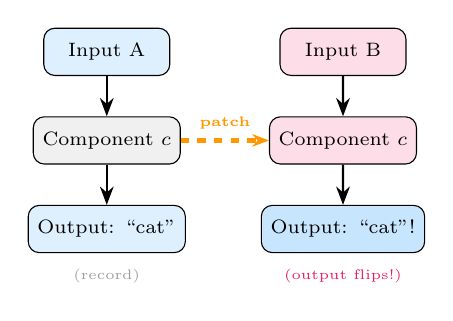
\begin{tikzpicture}[scale=0.75,
  box/.style={draw,rounded corners,minimum width=1.6cm,minimum height=0.6cm,font=\scriptsize,align=center}]

  % Model A
  \node[box,fill=evidence!15] (a1) at (0,4) {Input A};
  \node[box,fill=neutral!15] (a2) at (0,2.5) {Component $c$};
  \node[box,fill=evidence!15] (a3) at (0,1) {Output: ``cat''};
  \draw[-{Stealth},thick] (a1) -- (a2);
  \draw[-{Stealth},thick] (a2) -- (a3);

  % Model B
  \node[box,fill=choice!15] (b1) at (4,4) {Input B};
  \node[box,fill=choice!15] (b2) at (4,2.5) {Component $c$};
  \node[box,fill=evidence!25] (b3) at (4,1) {Output: ``cat''!};
  \draw[-{Stealth},thick] (b1) -- (b2);
  \draw[-{Stealth},thick] (b2) -- (b3);

  % Patch arrow
  \draw[causal,ultra thick,-{Stealth[length=6pt]},dashed] (a2.east) -- (b2.west)
    node[midway,above,font=\tiny\bfseries,causal] {patch};

  \node[font=\tiny,neutral] at (0,0.2) {(record)};
  \node[font=\tiny,choice] at (4,0.2) {(output flips!)};
\end{tikzpicture}

\vspace{0.5em}
{\small \textbf{Key insight:} patching maps causal structure, not just correlation. If patching component $X$ from trial A into trial B flips B's output, then $X$ \emph{causally carries} the information.}
\end{column}
\end{columns}
\end{frame}

%% --- SLIDE: Cross-region patching --- our version ---
\begin{frame}{Cross-region choice patching: activation patching for the brain}

\begin{columns}[T]
\begin{column}{0.53\textwidth}
{\small Instead of patching between \emph{components} of one network, we patch between \emph{brain regions} of one mouse:}

\vspace{0.2em}
{\small
\begin{enumerate}\setlength\itemsep{0.15em}
  \item Train a VAE per region $\to$ get $\mathbf{z}_{\text{choice}}$
  \item Take A's $\mathbf{z}_{\text{choice}}$ from a left-choice trial
  \item Patch into B's decoder on a right-choice trial
  \item Decode choice from B's patched representation
  \item Prediction flips $\to$ A, B share \textbf{compatible codes}
\end{enumerate}
}

\vspace{0.2em}
{\small \textbf{Directed}: A$\to$B may work but B$\to$A may not $\to$ reveals sender/receiver roles.}
\end{column}

\begin{column}{0.44\textwidth}
\textbf{What this tells us:}

\vspace{0.2em}
{\small
\begin{itemize}\setlength\itemsep{0.15em}
  \item Which regions share \textbf{compatible} choice representations
  \item \textbf{Directionality}: ``senders'' (code works elsewhere) vs ``receivers'' (accept external codes)
  \item A \textbf{circuit map} from representational compatibility, not anatomy
\end{itemize}
}

\vspace{0.2em}
{\small \textbf{Key difference from ML:} patching between \emph{separately trained} encoders --- compatibility reflects shared geometry, not shared weights.}
\end{column}
\end{columns}
\end{frame}

\section{9. Choice information flow}\hypertarget{sec:9}{}

%% --- SLIDE: Network graph ---
\begin{frame}{Choice information flow network}
\begin{columns}[T]
\begin{column}{0.55\textwidth}
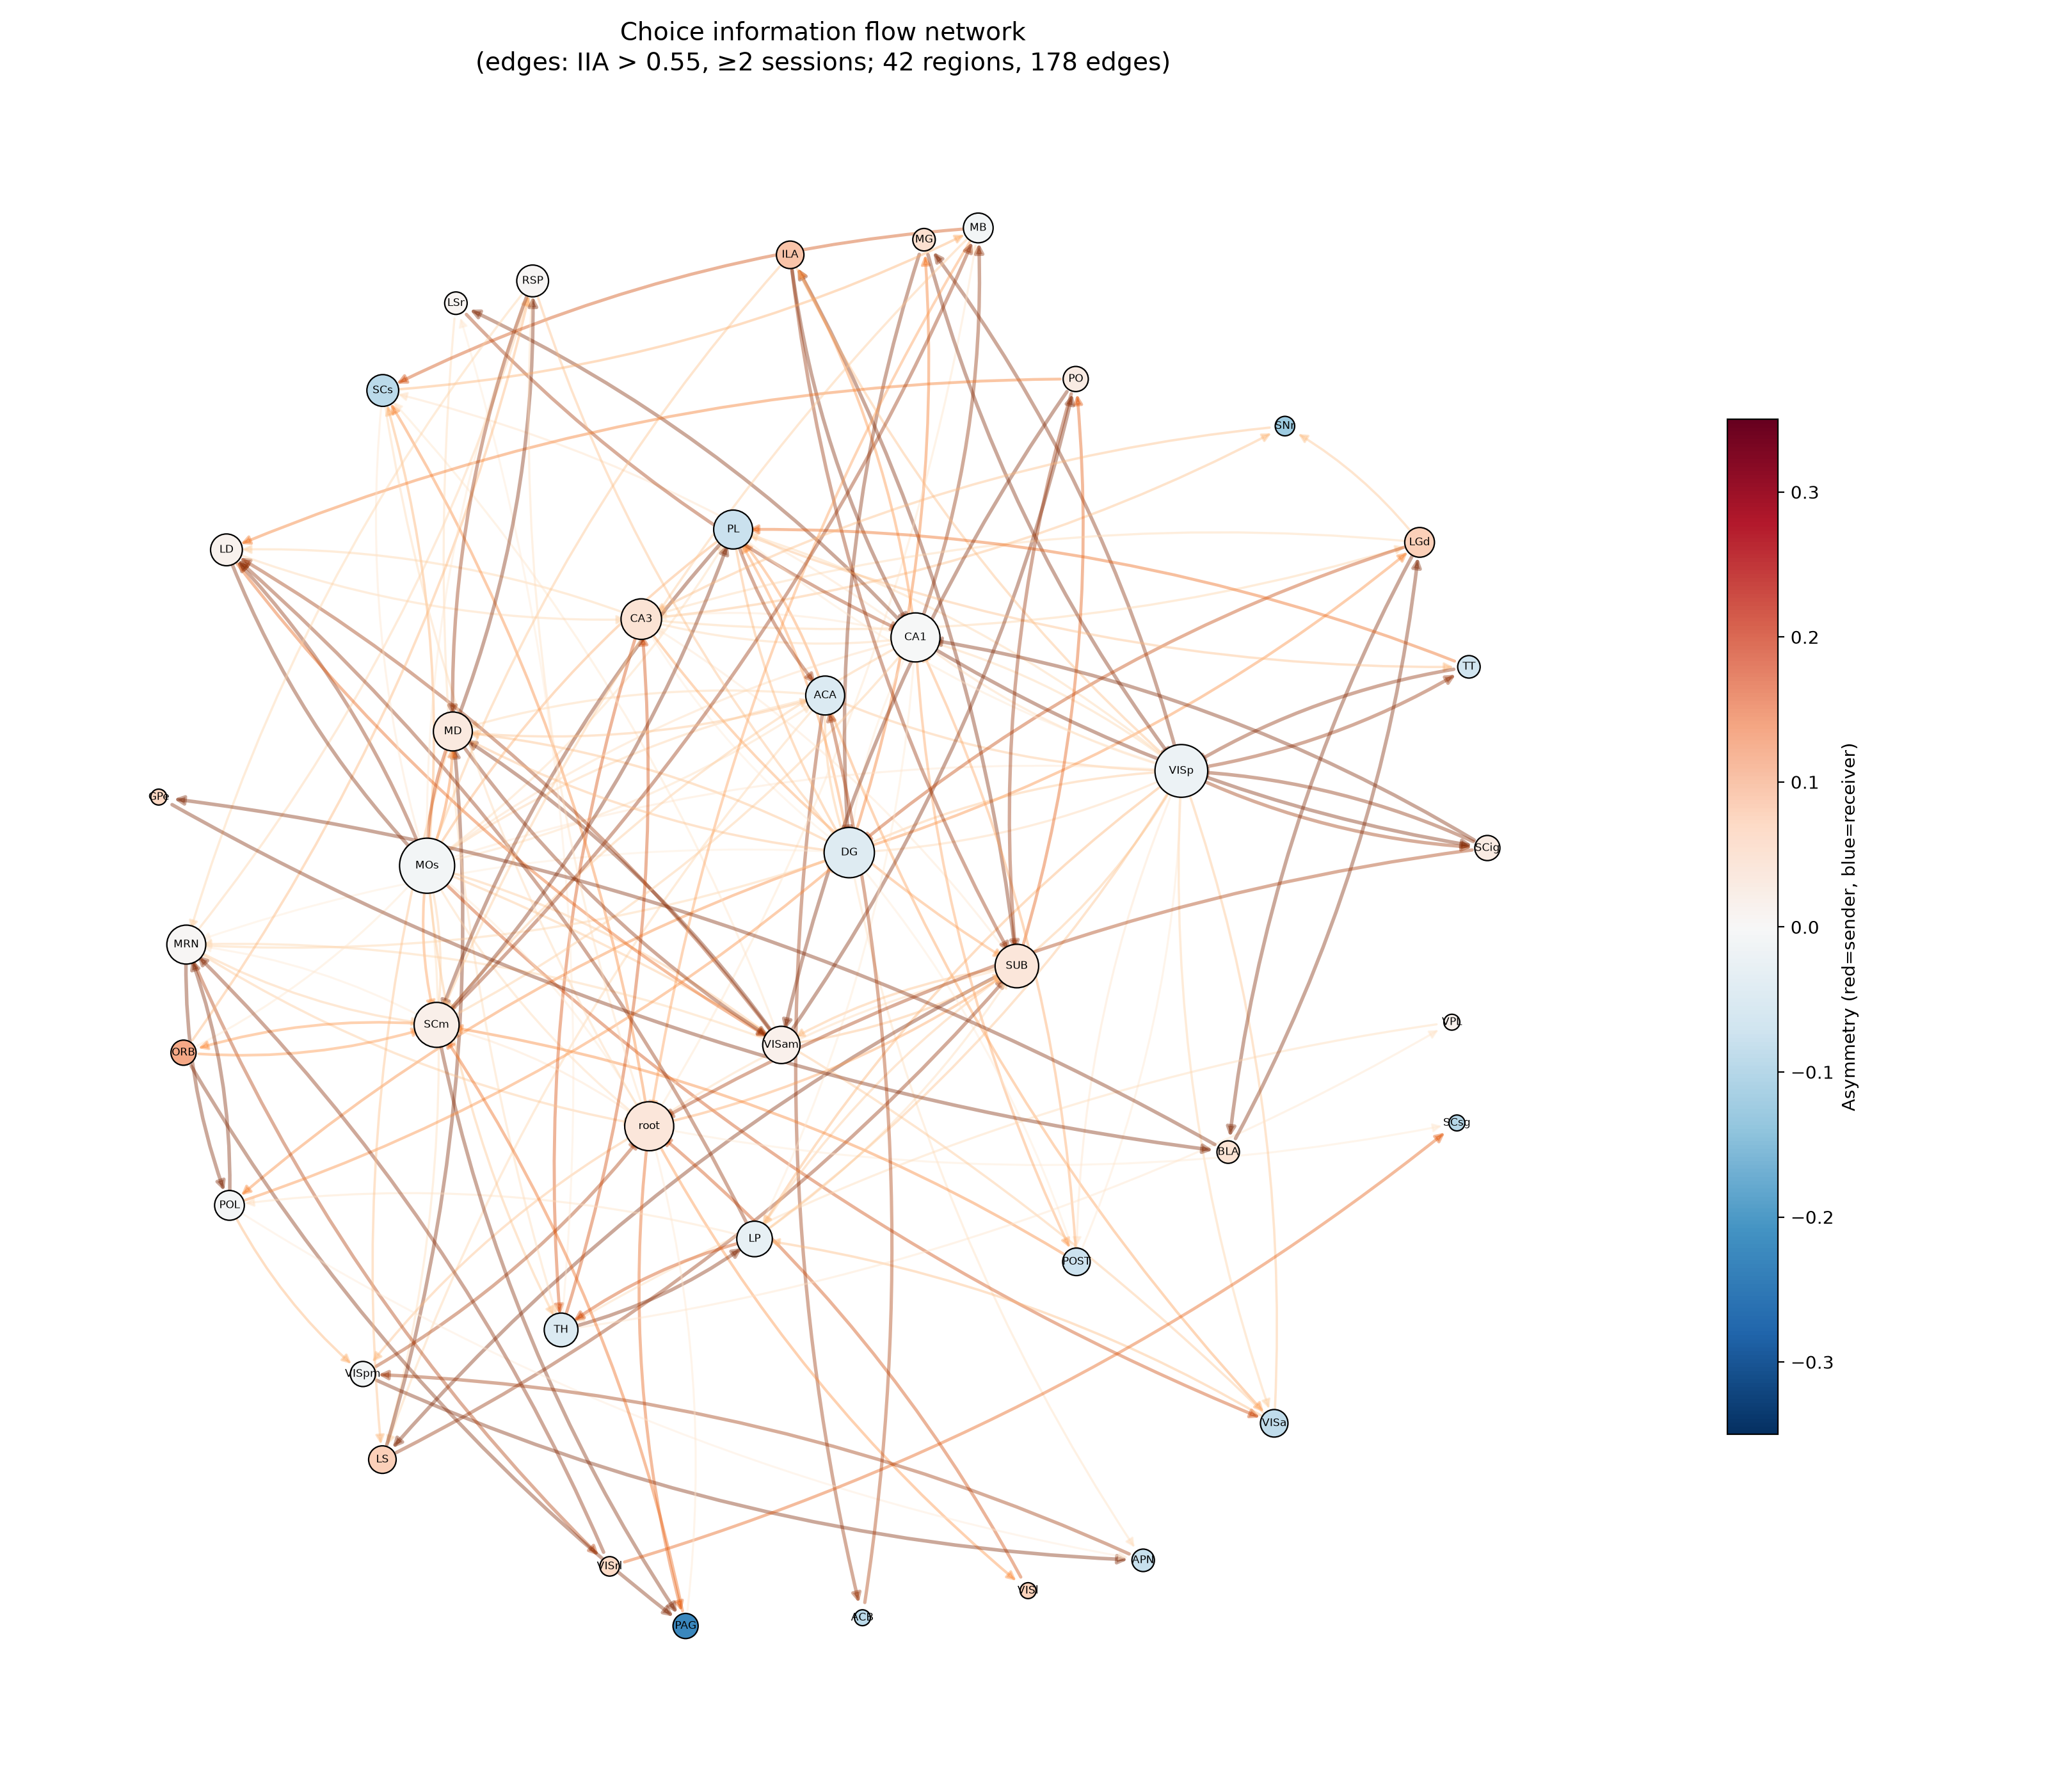
\includegraphics[width=\textwidth]{exp70_network_graph.png}
\end{column}
\begin{column}{0.43\textwidth}
\vspace{0.2em}
\textbf{Reading the graph:}

\vspace{0.2em}
{\small
\begin{itemize}\setlength\itemsep{0.1em}
  \item Each node is a brain region
  \item Directed edges: patching IIA $> 0.55$ (min.\ 2 sessions)
  \item Node size $\propto$ connection count
  \item \textcolor{red}{Red nodes} = net senders (outgoing $>$ incoming)
  \item \textcolor{blue}{Blue nodes} = net receivers (incoming $>$ outgoing)
  \item Edge color = IIA strength
\end{itemize}
}

\vspace{0.2em}
{\small \textbf{Key hubs:} ILA, LS, MD are strong senders. CA, ACB are strong receivers.}
\end{column}
\end{columns}
\end{frame}

%% --- SLIDE: Focused heatmap ---
\begin{frame}{Cross-region transfer: top 25 most connected regions}
\begin{columns}[T]
\begin{column}{0.55\textwidth}
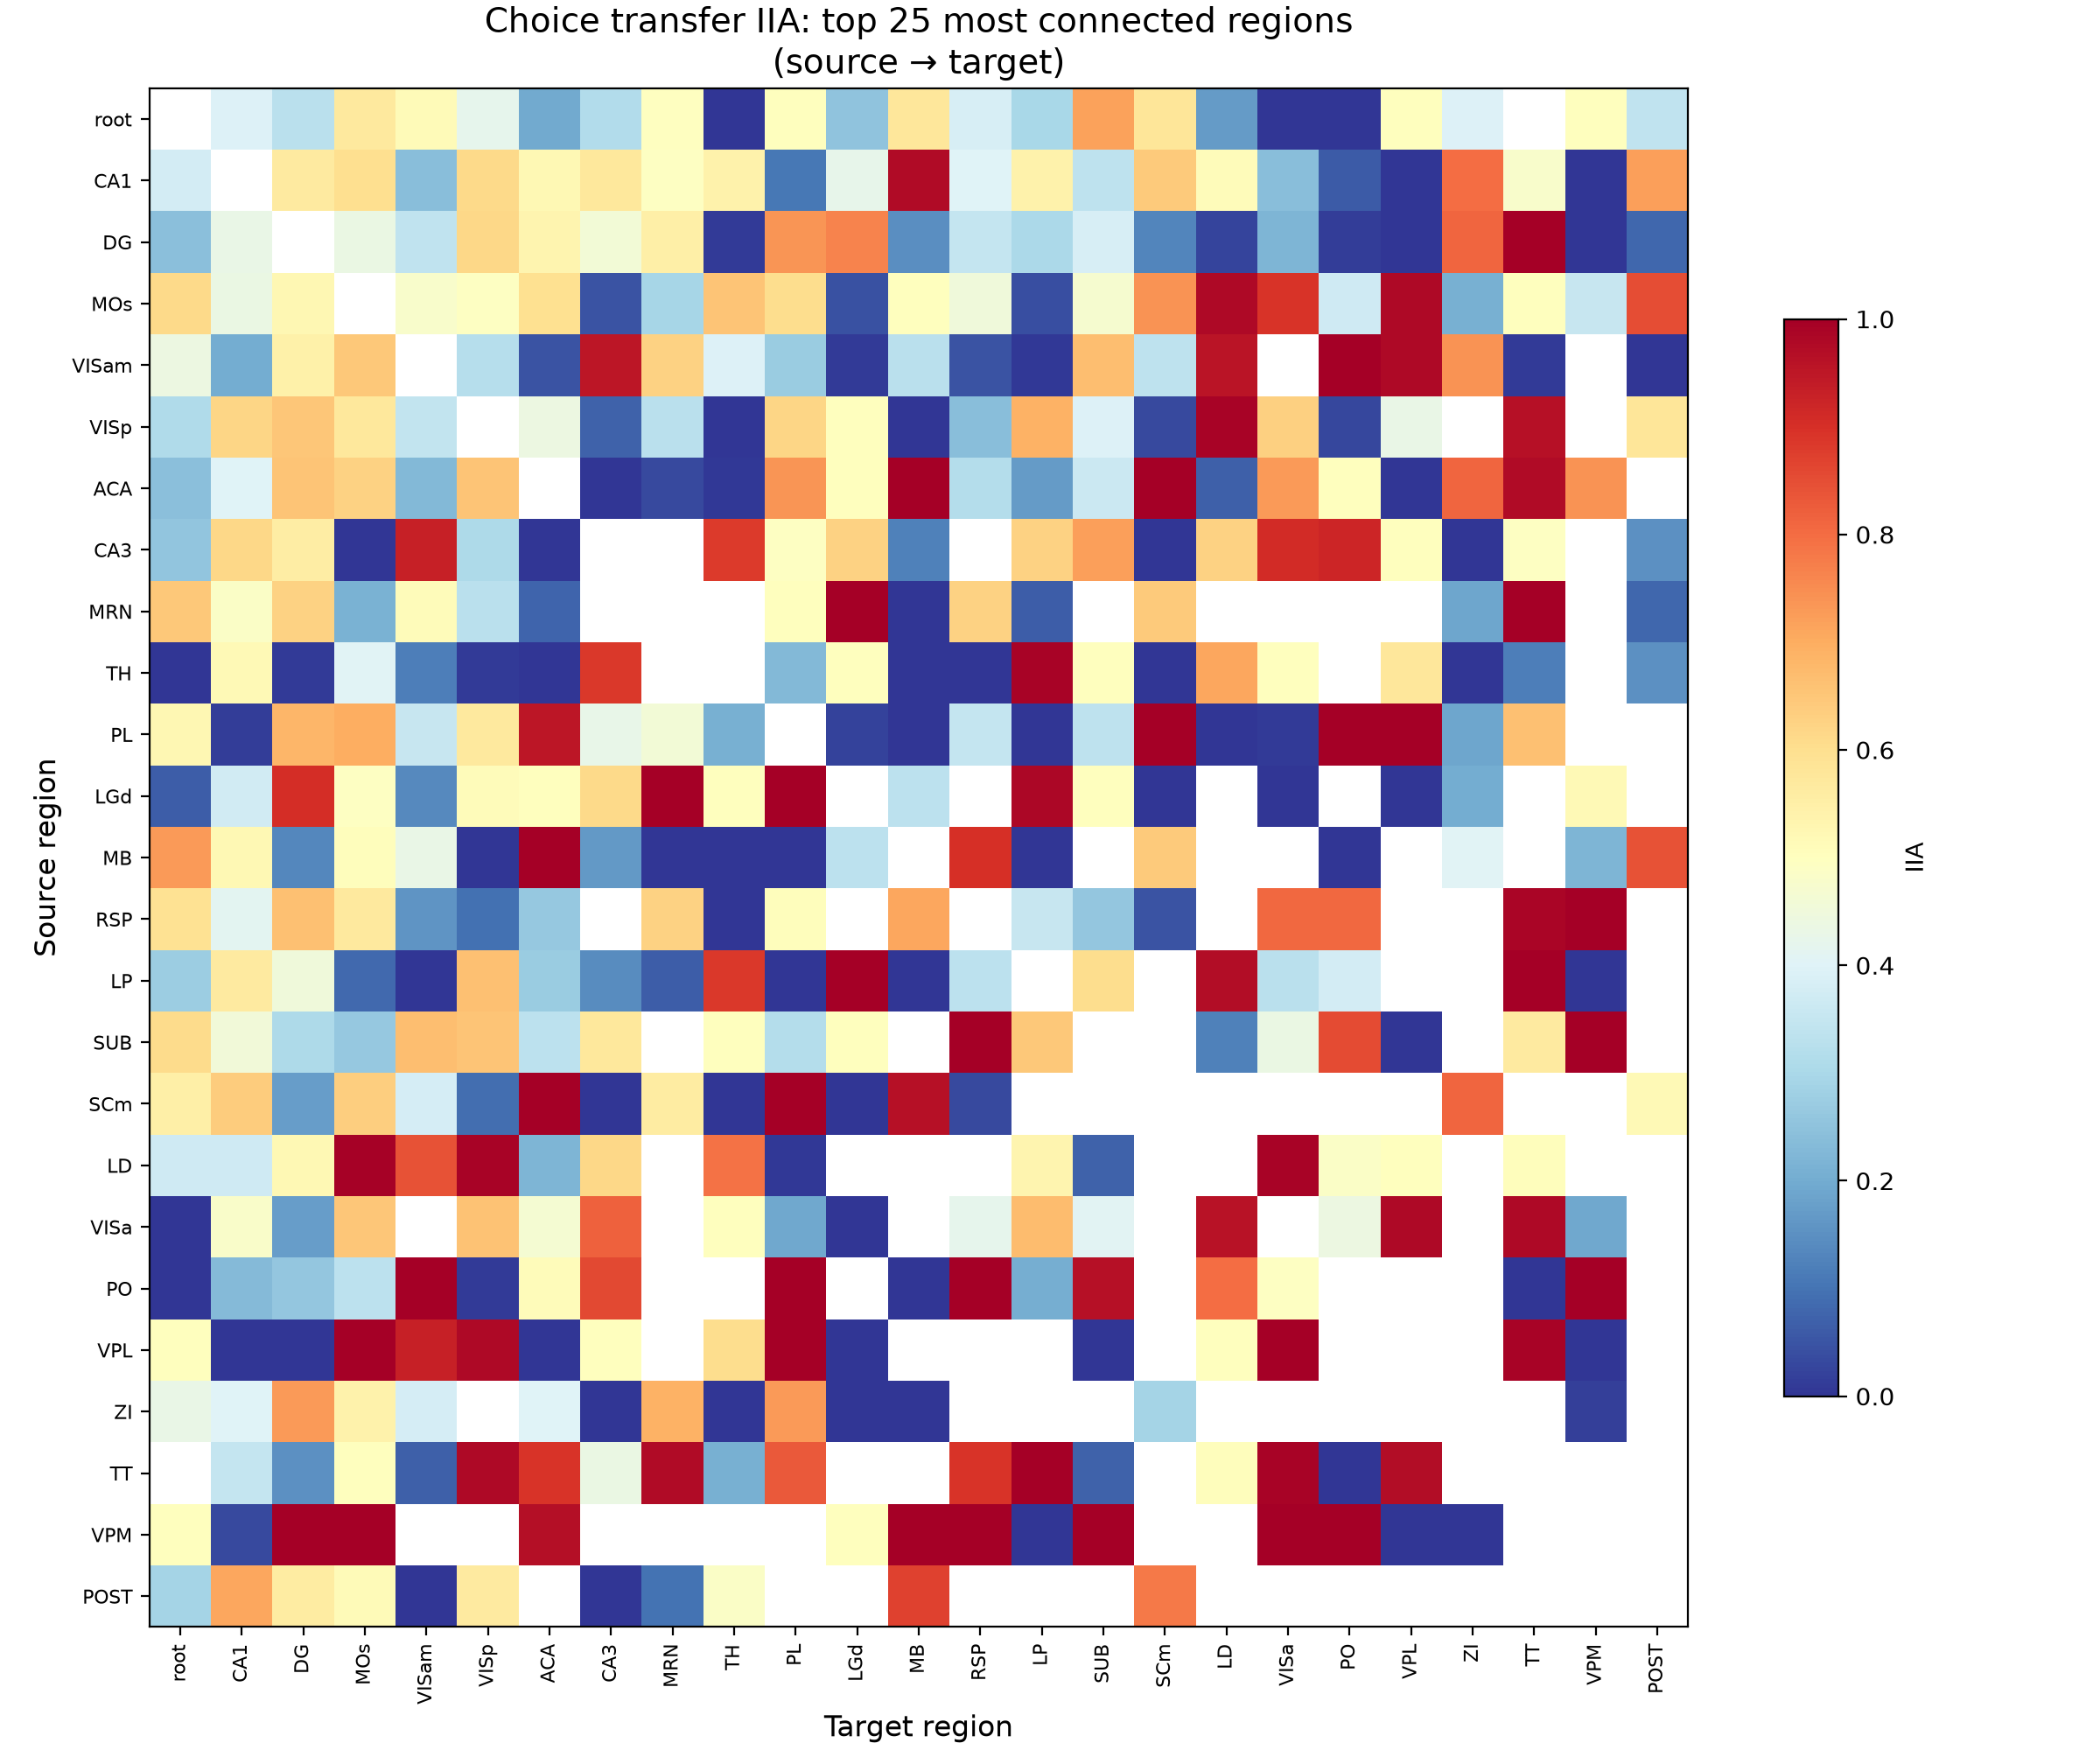
\includegraphics[width=\textwidth]{exp70_focused_heatmap.png}
\end{column}
\begin{column}{0.43\textwidth}
\vspace{0.2em}
\textbf{Reading the heatmap:}

\vspace{0.2em}
{\small
\begin{itemize}\setlength\itemsep{0.1em}
  \item Row = source region, column = target
  \item Color = IIA when patching source's $\mathbf{z}_{\text{choice}}$ into target
  \item \textcolor{red}{Red/yellow} = high transfer (compatible codes)
  \item \textcolor{blue}{Blue} = low transfer (incompatible)
  \item Gray = no co-recorded sessions
\end{itemize}
}

\vspace{0.3em}
{\small \textbf{Structure visible:} warm blocks reveal groups sharing compatible choice representations. The matrix is \emph{not symmetric} --- transfer is directional.}
\end{column}
\end{columns}
\end{frame}

%% --- SLIDE: Hub roles ---
\begin{frame}{Sender and receiver hubs in the choice network}
\begin{columns}[T]
\begin{column}{0.55\textwidth}
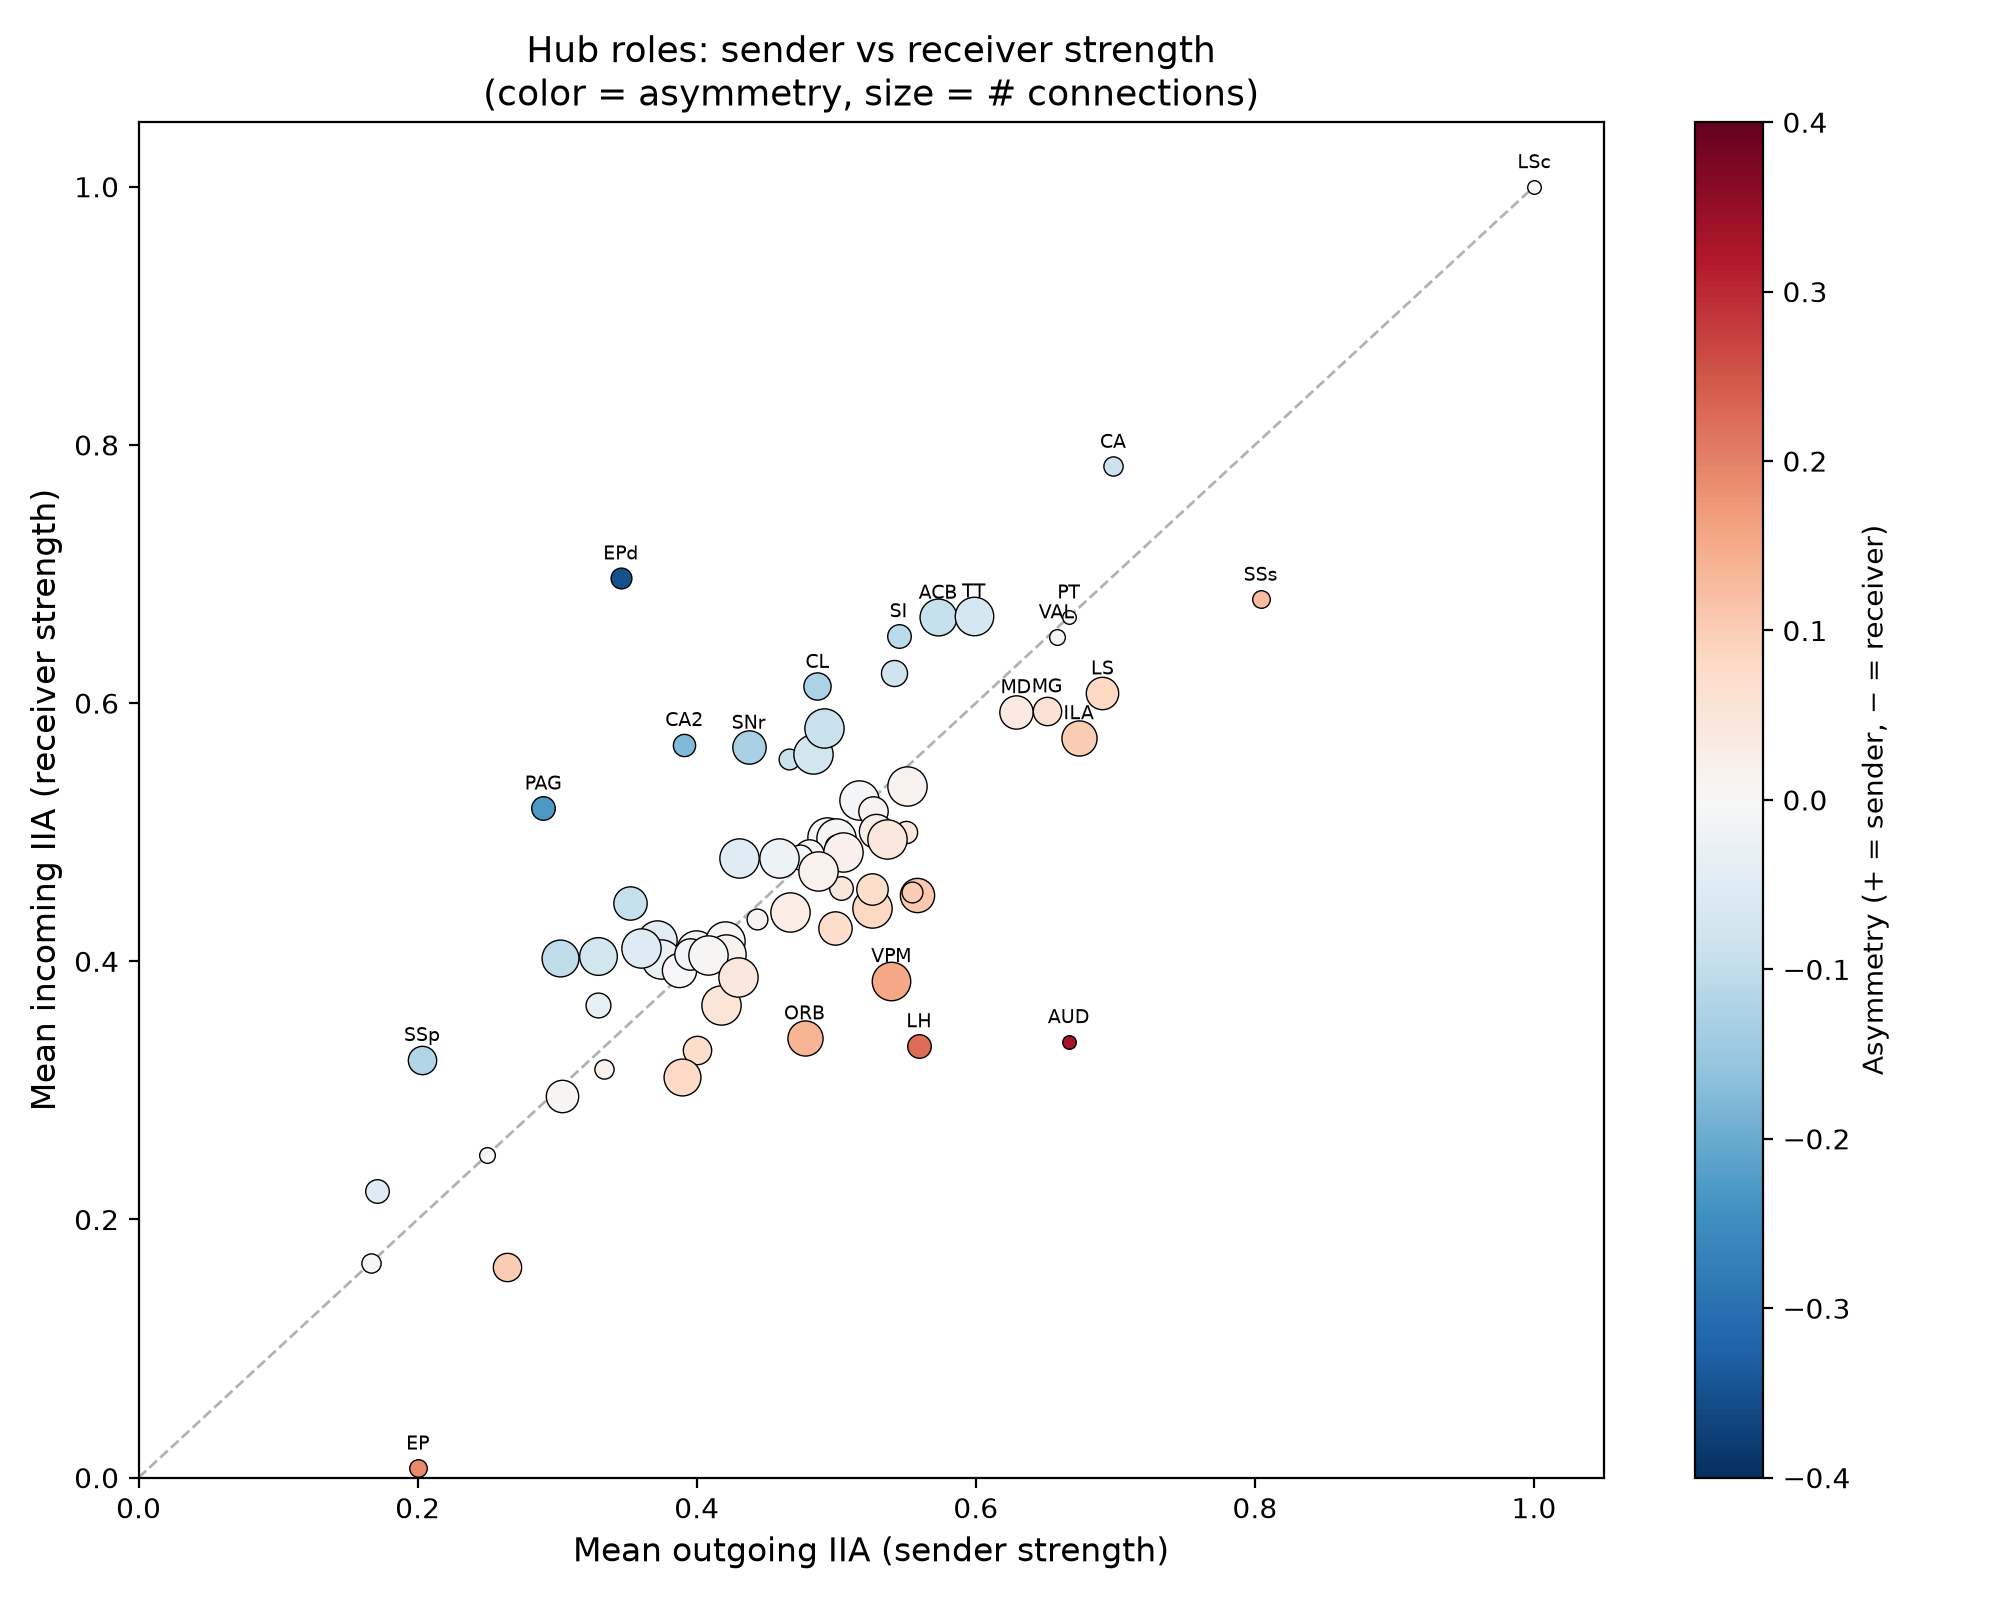
\includegraphics[width=\textwidth]{exp70_hub_scatter.png}
\end{column}
\begin{column}{0.43\textwidth}
\vspace{0.2em}
\textbf{Reading the scatter:}

\vspace{0.2em}
{\small
\begin{itemize}\setlength\itemsep{0.1em}
  \item $x$-axis: how well a region's code \emph{transfers out} (sender)
  \item $y$-axis: how well it \emph{accepts} external codes (receiver)
  \item Diagonal = symmetric; above = net receiver; below = net sender
  \item Dot size $\propto$ number of connections
\end{itemize}
}

\vspace{0.2em}
{\small \textbf{Notable asymmetries:} AUD is a strong sender ($+0.33$), EPd a strong receiver ($-0.35$), ILA the strongest sender ($0.67$ out). May reflect feedforward flow from sensory $\to$ decision regions.}
\end{column}
\end{columns}
\end{frame}

%% ============================================================
%% PART 4: ADDITIONAL TESTING
%% ============================================================

\begin{frame}[plain]
\vfill
\begin{center}
  \setlength{\fboxrule}{2.5pt}%
  \fcolorbox{black}{white}{\parbox{0.7\textwidth}{\centering\vspace{0.8em}
    {\Large\bfseries Part 4}\\[0.5em]
    {\large Additional testing}
  \vspace{0.8em}}}
\end{center}
\vfill
\end{frame}

\begin{frame}{In this section}
\begin{columns}[T]
\begin{column}{0.3\textwidth}
\textbf{10. Per-variable causal subspaces}\\[0.2em]
{\small 4 task variables each get their own causal subspace with non-trivial IIA. The VAE decomposition generalizes beyond binary choice.}
\end{column}
\begin{column}{0.3\textwidth}
\textbf{11. Optogenetic: linear vs nonlinear}\\[0.2em]
{\small Full method comparison against silencing ground truth. LDA is actively misleading ($\rho = -0.82$); VAE and decoding are not.}
\end{column}
\begin{column}{0.3\textwidth}
\textbf{12. Encoder specialization}\\[0.2em]
{\small The structured VAE develops dedicated choice-detector channels. Specialization emerges from the bottleneck.}
\end{column}
\end{columns}
\end{frame}

\section{10. Per-variable causal subspaces}\hypertarget{sec:10}{}

%% --- SLIDE: Multi-task ---
\begin{frame}{Four task variables, four distinct subspaces}
\begin{columns}[T]
\begin{column}{0.50\textwidth}
\textbf{Question:} Does the subspace approach generalize beyond binary choice?

\vspace{0.5em}
\textbf{Method:} Train structured VAEs for 4 task variables: choice (left/right), stimulus contrast, reaction time, and feedback (correct/incorrect). Each gets its own 3-dim subspace.

\vspace{0.5em}
\textbf{Result:} All 4 variables produce distinct, structured subspaces with non-trivial IIA. The subspaces are geometrically separable --- not a single ``task-general'' axis.
\end{column}

\begin{column}{0.47\textwidth}
\vspace{0.5em}
{\small
\textbf{Why this matters:}
\begin{itemize}\setlength\itemsep{0.3em}
  \item Rules out the objection that IIA only works for binary left/right
  \item Shows the geometric decomposition is general, not task-specific
  \item Different variables occupy different subspaces within the same neural population
  \item The structured VAE architecture works for continuous variables too (contrast, RT), not just binary classification
\end{itemize}
}
\end{column}
\end{columns}
\end{frame}

%% --- SLIDE: Per-variable IIA results ---
\begin{frame}{VAE outperforms LDA across all task variables}
\begin{columns}[T]
\begin{column}{0.55\textwidth}
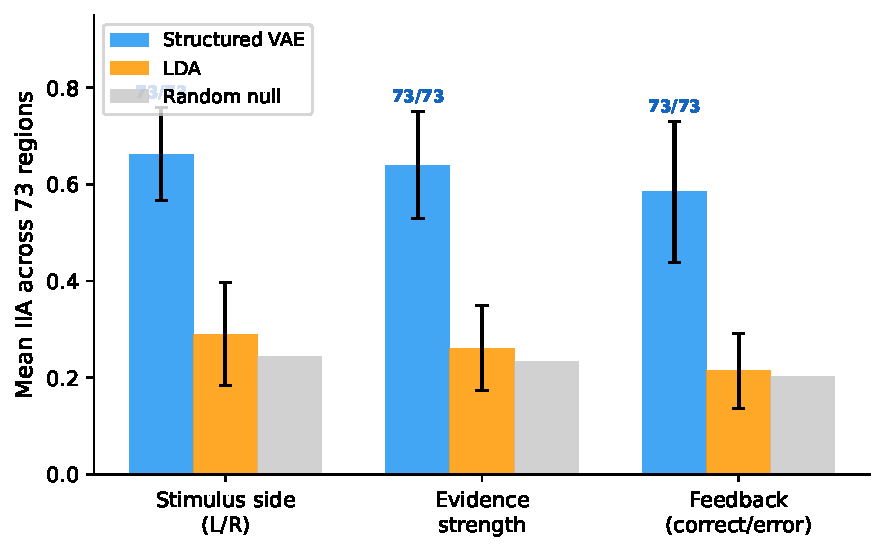
\includegraphics[width=\textwidth]{per_variable_iia.pdf}
\end{column}
\begin{column}{0.42\textwidth}
\vspace{0.3em}
{\small
\begin{itemize}\setlength\itemsep{0.3em}
  \item VAE beats LDA in \textbf{73/73 regions} for every variable
  \item Stimulus side (IIA $= 0.66$), evidence strength ($0.64$), feedback ($0.58$) --- all well above null ($\sim 0.23$)
  \item LDA barely exceeds random for any variable
  \item The structured decomposition works for continuous variables too, not just binary classification
\end{itemize}
}
\end{column}
\end{columns}
\end{frame}

\section{11. Optogenetic ground truth: linear vs nonlinear}\hypertarget{sec:11}{}

%% --- SLIDE: Optogenetic scatter ---
\begin{frame}{LDA is anti-correlated with causal importance}
\begin{columns}[T]
\begin{column}{0.50\textwidth}
{\small \textbf{The external test:} Zatka-Haas et al.\ (2021) silenced cortical regions with optogenetics and measured behavioral impact. This is \textbf{ground-truth causal importance} --- completely independent of our geometry pipeline.}

\vspace{0.3em}
{\small \textbf{Result:} LDA IIA is \emph{negatively} correlated with silencing effect. Regions where LDA says choice information is strongest are the ones where silencing has the \emph{least} effect.}

\vspace{0.3em}
{\small The VAE trend is in the right direction but underpowered at $n = 7$.}
\end{column}

\begin{column}{0.48\textwidth}
\vspace{-0.3em}
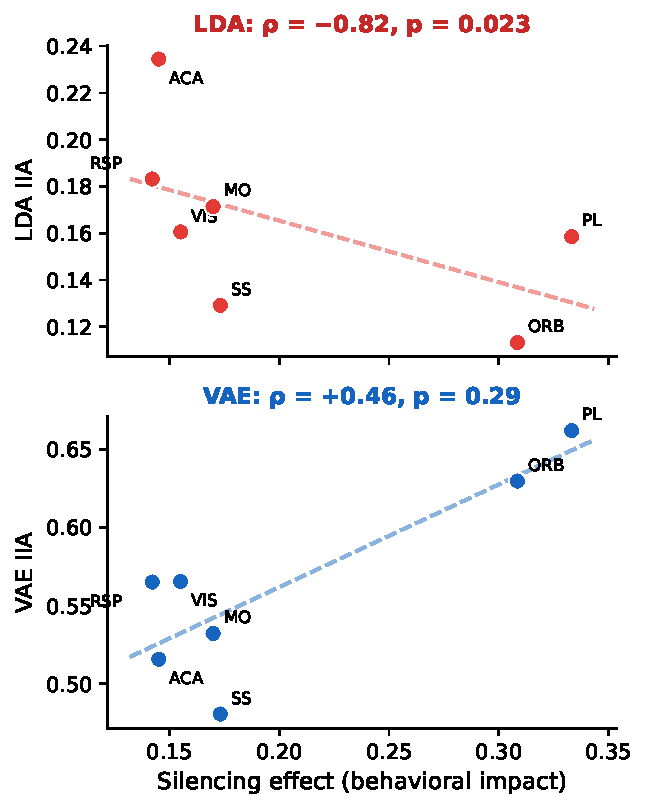
\includegraphics[width=\textwidth]{lda_vae_vs_silencing.pdf}
\end{column}
\end{columns}
\end{frame}

%% --- SLIDE: Optogenetic full stats ---
\begin{frame}{Full optogenetic validation: bootstrap CIs and permutation tests}

\vspace{-0.3em}
{\scriptsize Spearman rank, $n = 7$ grouped cortical regions (12 sub-regions grouped by Allen CCF parent). Bootstrap: 10k resamples, BCa CIs. Permutation: 10k shuffles.}

\vspace{0.2em}
\begin{center}
{\scriptsize
\begin{tabular}{lcccc}
\toprule
\textbf{Method} & \textbf{$\rho$} & \textbf{$p$} & \textbf{Bootstrap CI} & \textbf{Perm.\ $p$} \\
\midrule
LDA IIA & $\mathbf{-0.82}$ & $\mathbf{0.023}$ & $[-1.00, -0.41]$ & $0.036$ \\
VAE IIA & $+0.46$ & $0.29$ & $[-0.70, +1.00]$ & $0.30$ \\
IIA above null & $+0.68$ & $0.094$ & $[-0.22, +1.00]$ & $0.11$ \\
\bottomrule
\end{tabular}
}
\end{center}

\vspace{0.2em}
\begin{columns}[T]
\begin{column}{0.48\textwidth}
{\small \textbf{Key points:}
\begin{itemize}\setlength\itemsep{0.1em}
  \item LDA bootstrap CI excludes zero --- robust
  \item LDA permutation $p$ also significant ($0.036$)
  \item VAE CI spans zero --- underpowered, not contradicted
  \item IIA above null trends positive ($p = 0.094$)
\end{itemize}
}
\end{column}
\begin{column}{0.48\textwidth}
{\small \textbf{Limitations:}
\begin{itemize}\setlength\itemsep{0.1em}
  \item Small $n$ ($= 7$ groups) limits power
  \item Silencing data from different mice/lab
  \item Grouping assumes Allen CCF hierarchy
  \item More silencing sites would sharpen all CIs
\end{itemize}
}
\end{column}
\end{columns}
\end{frame}

\section{12. Encoder specialization}\hypertarget{sec:12}{}

%% --- SLIDE: VAE encoder specialization ---
\begin{frame}{The encoder develops specialized choice detectors}
\begin{columns}[T]
\begin{column}{0.50\textwidth}
\textbf{Question:} Does the structured VAE learn interpretable internal structure, or is it a black box that happens to score well?

\vspace{0.5em}
\textbf{Method:} Channel Expertise Score (CES) measures how specialized each encoder channel is for choice vs.\ nuisance information.

\vspace{0.5em}
\textbf{Result:} Choice channels are \textbf{2.7$\times$ more specialized} than nuisance channels. Random splits give a ratio of 1.0.
\end{column}

\begin{column}{0.47\textwidth}
\vspace{0.5em}
{\small
\begin{tabular}{lc}
\toprule
\textbf{Metric} & \textbf{Value} \\
\midrule
CES choice channels & 0.077 \\
CES other channels & 0.028 \\
\textbf{Choice/other ratio} & \textbf{2.73} \\
Random split ratio & 1.005 \\
Structured vs random lift & 2.72$\times$ \\
\bottomrule
\end{tabular}
}

\vspace{0.5em}
{\small The structural bottleneck doesn't just improve IIA scores---it forces the encoder to develop specialized channels. The architecture creates interpretability.}
\end{column}
\end{columns}
\end{frame}

%% --- SLIDE: Encoder specialization by region ---
\begin{frame}{Channel specialization across brain regions}
\begin{columns}[T]
\begin{column}{0.50\textwidth}
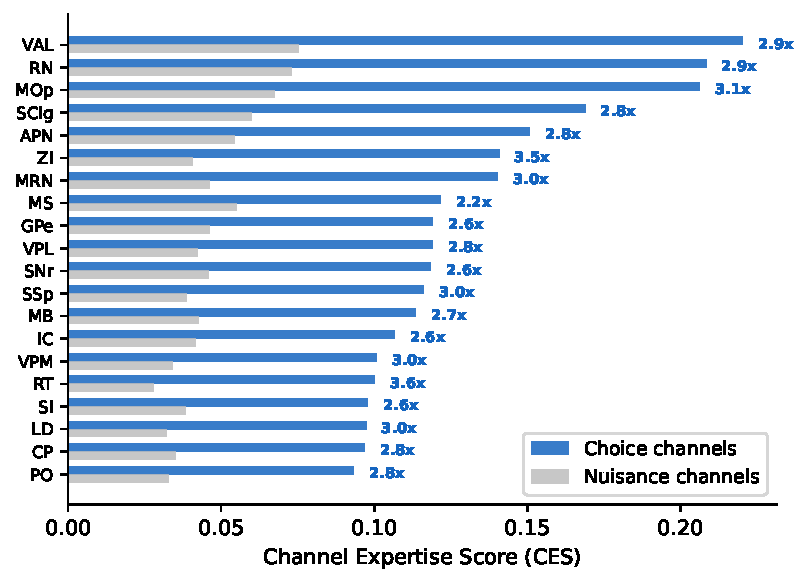
\includegraphics[width=\textwidth]{encoder_specialization.pdf}
\end{column}
\begin{column}{0.47\textwidth}
\vspace{0.3em}
{\small
\begin{itemize}\setlength\itemsep{0.2em}
  \item \textbf{Every region} shows choice channels more specialized than nuisance (ratio $2.1$--$3.6\times$)
  \item Motor regions (MOp, VAL, RN) have the highest absolute CES --- consistent with choice $\to$ action readout
  \item Sensory regions (VIS, AUD) specialize less but still $> 2.5\times$
  \item Specialization is not an artifact of the bottleneck: random channel splits give ratio $= 1.0$
\end{itemize}
}
\end{column}
\end{columns}
\end{frame}

%% --- SLIDE: Deeper encoder analysis ---
\begin{frame}{What do the channels actually learn?}
\begin{columns}[T]
\begin{column}{0.42\textwidth}
\vspace{-0.3em}
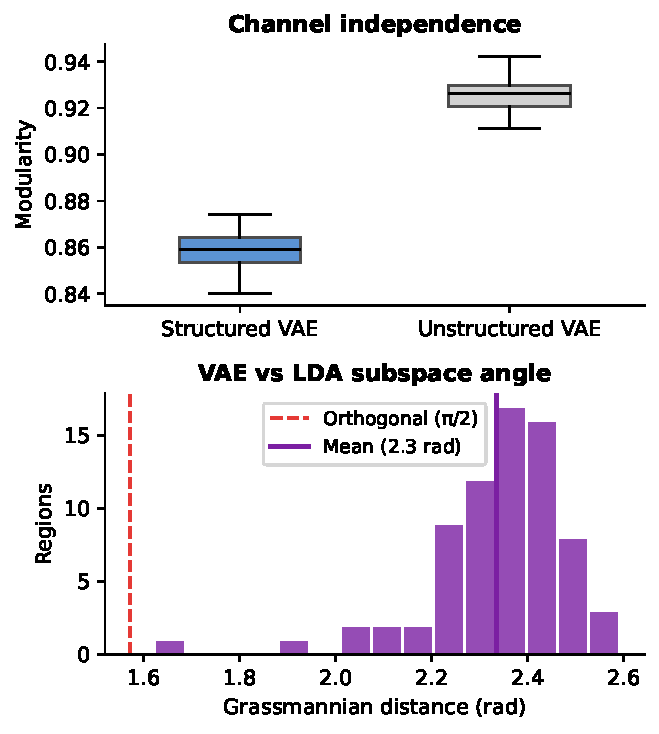
\includegraphics[width=\textwidth]{encoder_deep_analysis.pdf}
\end{column}
\begin{column}{0.55\textwidth}
\vspace{0.3em}
{\small \textbf{Channel independence} (top):}

\vspace{0.2em}
{\small Structured VAE has lower modularity (0.86) than unstructured (0.93). The bottleneck forces choice and nuisance channels to carry \emph{non-overlapping} information --- channels specialize rather than redundantly encoding the same signal.}

\vspace{0.5em}
{\small \textbf{VAE vs LDA subspace angle} (bottom):}

\vspace{0.2em}
{\small VAE and LDA find completely different subspaces. Mean Grassmannian distance $= 2.3$ rad, well past orthogonal ($\pi/2 = 1.57$). The VAE is not rediscovering LDA --- it finds directions LDA cannot access because they require nonlinear separation.}
\end{column}
\end{columns}
\end{frame}

\section{13. SAE-style inductive bias ablation}\hypertarget{sec:13}{}

%% --- SLIDE: SAE ablation ---
\begin{frame}{Overcomplete sparse representations improve causal subspaces}
\begin{columns}[T]
\begin{column}{0.52\textwidth}
\vspace{-0.3em}
\includegraphics[width=\textwidth]{exp73_sae_ablation.pdf}
\end{column}
\begin{column}{0.45\textwidth}
\vspace{0.3em}
{\small \textbf{Question:} Which inductive biases matter for finding causal subspaces in neural populations?}

\vspace{0.3em}
{\small \textbf{Ablation:} 6 models $\times$ 73 regions. Three biases tested:
\begin{enumerate}\setlength\itemsep{0.1em}
  \item Structured split ($z_{\text{choice}}$ / $z_{\text{other}}$)
  \item Label-conditional prior ($\pi$-VAE style)
  \item Overcomplete $z_{\text{choice}}$ ($8\times$) + L1 sparsity
\end{enumerate}
}

\vspace{0.3em}
{\small \textbf{Result:} SAE-style sparsity is the winning ingredient. All three SAE variants beat all three VAE variants. The label-conditional prior that works on transformer representations \emph{hurts slightly} on neural data.}

\vspace{0.3em}
{\small Best: \textbf{SAE Structured} (split + overcomplete + L1) at IIA $= 0.962$, vs.\ structured VAE baseline $= 0.939$.}
\end{column}
\end{columns}
\end{frame}

%% --- SLIDE: Validity scorecard for IIA paper ---
\begin{frame}{Validity scorecard: IIA in biological neural populations}
\vspace{-0.5em}
{\scriptsize
\begin{tabular}{lp{7cm}c}
\toprule
\textbf{Criterion} & \textbf{Evidence} & \textbf{Status} \\
\midrule
\textbf{Necessity} & Swapping choice subspace flips prediction ($2.3\times$ above random) & \textcolor{pass}{\textbf{Pass}} \\
\textbf{Sufficiency} & Choice subspace alone decodes better than full activity ($1.16\times$) & \textcolor{pass}{\textbf{Pass}} \\
\textbf{Specificity} & Only choice axis flips; RT, feedback, random do not & \textcolor{pass}{\textbf{Pass}} \\
\textbf{Confound control} & Neuron count, firing rate, temporal shuffle: no confound $> 0.5$ & \textcolor{pass}{\textbf{Pass}} \\
\textbf{Graded response} & IIA monotonic in 70\% of regions under dimension ablation & \textcolor{pass}{\textbf{Pass}} \\
\textbf{VAE $>$ LDA} & VAE wins 73/73 regions ($3.4\times$); VAE subspace $\perp$ LDA & \textcolor{pass}{\textbf{Pass}} \\
\textbf{Multi-task} & 4 variables, 4 distinct subspaces, VAE wins 73/73 each & \textcolor{pass}{\textbf{Pass}} \\
\textbf{Engagement control} & $\mathbf{z}_{\text{engage}} \perp \mathbf{z}_{\text{choice}}$; cross-IIA only 17\% & \textcolor{pass}{\textbf{Pass}} \\
\textbf{External validation} & LDA anti-correlated with silencing ($\rho = -0.82$, $p = 0.023$) & \textcolor{pass}{\textbf{Pass}} \\
\textbf{Circuit structure} & 1,438 directed pairs; sender/receiver hubs in 73 regions & \textcolor{pass}{\textbf{Pass}} \\
\textbf{Encoder interpretability} & Choice channels $2.7\times$ more specialized; not rediscovering LDA & \textcolor{pass}{\textbf{Pass}} \\
\midrule
\textbf{IIA vacuity} & Nonlinear VAE achieves IIA $= 0.70$ on \emph{random noise} & \textcolor{fail}{\textbf{Fail}} \\
\bottomrule
\end{tabular}
}

\vspace{0.3em}
{\small 11 pass, 1 fail. The vacuity result is real --- nonlinear IIA can be gamed. External validation (optogenetics) is what saves the claim.}
\end{frame}

\section{Conclusions}

%% --- SLIDE: Limitations ---
\begin{frame}{Project limitations}
\begin{columns}[T]
\begin{column}{0.5\textwidth}
\textbf{Hard limits:}
\begin{itemize}
  \item \textbf{One task paradigm} (visual decision-making) --- 4 variables help but still one paradigm
  \item \textbf{Small silencing overlap}: $n = 7$ grouped regions --- CIs cannot shrink without more silencing data
  \item \textbf{IIA vacuity is real}: VAE achieves IIA $= 0.70$ on random noise --- external validation is load-bearing
  \item \textbf{Two datasets} (Steinmetz + Zatka-Haas silencing) but same species, same task family
\end{itemize}
\end{column}
\begin{column}{0.48\textwidth}
\textbf{Addressable with more compute:}
\begin{itemize}
  \item \textbf{Cross-region patching}: bootstrap over session subsets for edge stability
  \item \textbf{VAE training variance}: ensembles of multiple seeds per region
  \item \textbf{IBL replication}: same pipeline, different dataset --- in progress
  \item \textbf{More silencing sites}: would tighten all optogenetic CIs beyond $n = 7$
\end{itemize}
\end{column}
\end{columns}
\end{frame}

%% --- SLIDE: Summary ---
\begin{frame}{Summary: what we found and what it means}
\begin{columns}[T]
\begin{column}{0.5\textwidth}
\textbf{Established findings:}
\begin{enumerate}
  \item Evidence subspace causally mediates choice (4 intervention methods agree, $r = 0.78$)
  \item Learned subspaces 3.4$\times$ more causal than LDA (73/73 regions)
  \item Engagement and choice are separable ($\perp$ subspaces)
  \item 4 task variables have distinct geometric representations
  \item Directed circuit map reveals sender/receiver hub structure
\end{enumerate}
\end{column}
\begin{column}{0.48\textwidth}
\textbf{Critical nuances:}
\begin{enumerate}
  \setcounter{enumi}{5}
  \item \textcolor{fail}{IIA is vacuous for nonlinear methods}---VAE fits random noise equally well
  \item \textcolor{pass}{But:} LDA is \emph{anti-correlated} with optogenetic causal importance ($\rho = -0.82$, $p = 0.023$)---this is external and not vacuous
  \item Encoder channels develop $2.7\times$ specialization; VAE subspaces are geometrically distant from LDA ($2.3$ rad)
\end{enumerate}

\vspace{0.3em}
{\small \textbf{Takeaway:} External validation anchors IIA claims. The structured VAE provides the right balance of flexibility and constraint.}
\end{column}
\end{columns}
\end{frame}

%% --- SLIDE: Conclusion ---
\begin{frame}{Conclusion}

\begin{center}
\vspace{0.5em}
{\Large Mechanistic interpretability tools \textbf{can} be applied}

\vspace{0.2em}

{\Large to biological neural recordings ---}

\vspace{0.6em}

{\Large but \textbf{IIA is vacuous} for nonlinear models}

\vspace{0.2em}

{\Large without external ground truth.}

\vspace{1.2em}

{\small Learned subspaces recover 3.4$\times$ more signal than linear methods,}

\vspace{0.2em}

{\small but every nonlinear method that outperformed linear baselines also fit to noise.}

\vspace{0.1em}

{\small Only optogenetic validation and engagement controls separated signal from overfitting.}
\end{center}
\end{frame}

%% --- SLIDE: Thank you ---
\begin{frame}{Thank you}

\textbf{Paper:} TBD

\vspace{0.3em}
\textbf{Repository:} \href{https://github.com/elliottower/causal-geometry-neuro}{\texttt{github.com/elliottower/causal-geometry-neuro}}

\vspace{0.3em}
\textbf{Contact:} \texttt{elliot@elliottower.com}

\vspace{0.3em}
{\small
\textbf{Data sources:}
\begin{itemize}\setlength\itemsep{0pt}
  \item \href{https://doi.org/10.1038/s41586-019-1787-x}{Steinmetz et al.\ 2019} --- 73 brain regions, 39 sessions, 10 mice, ${\sim}30{,}000$ neurons (Neuropixels)
  \item \href{https://doi.org/10.7554/eLife.63163}{Zatka-Haas et al.\ 2021} --- optogenetic silencing, 52 coordinates, 26 cortical sites (Figshare)
  \item \href{https://connectivity.brain-map.org/}{Allen Mouse Brain Atlas} --- structural connectivity for anatomy control
\end{itemize}

\textbf{Experiments:} 72 experiments, Modal A10G GPUs
}
\end{frame}

%% --- SLIDE: References (1/2) ---
\begin{frame}{References (1/2)}
\vspace{-0.3em}
{\scriptsize
\begin{itemize}\setlength\itemsep{0pt}
  \item Arbour et al.\ (2016). \href{https://www.auai.org/uai2016/proceedings/papers/217.pdf}{Inferring causal direction from relational data.} UAI.
  \item Craver (2007). \href{https://doi.org/10.1093/acprof:oso/9780199299317.001.0001}{Explaining the Brain.} Oxford University Press.
  \item Esmaeili et al.\ (2019). \href{https://proceedings.mlr.press/v89/esmaeili19a}{Structured disentangled representations.} AISTATS.
  \item Geiger et al.\ (2024). \href{https://arxiv.org/abs/2303.02536}{Finding alignments between interpretable causal variables and distributed neural representations.} arXiv.
  \item Maier et al.\ (2013). \href{https://arxiv.org/abs/1309.6843}{A sound and complete algorithm for learning causal models from relational data.} UAI.
  \item Mayo (2018). \href{https://doi.org/10.1017/9781107286184}{Statistical Inference as Severe Testing.} Cambridge University Press.
  \item Musall et al.\ (2019). \href{https://doi.org/10.1038/s41593-019-0502-4}{Single-trial neural dynamics are dominated by richly varied movements.} \textit{Nature Neuroscience}.
  \item Narayanaswamy et al.\ (2017). \href{https://arxiv.org/abs/1706.00400}{Learning disentangled representations with semi-supervised deep generative models.} NeurIPS.
\end{itemize}
}
\end{frame}

%% --- SLIDE: References (2/2) ---
\begin{frame}{References (2/2)}
\vspace{-0.3em}
{\scriptsize
\begin{itemize}\setlength\itemsep{0pt}
  \item Pearl \& Bareinboim (2011). \href{https://arxiv.org/abs/1203.3519}{Transportability of causal and statistical relations.} AAAI.
  \item Shallice (1988). \href{https://doi.org/10.1017/CBO9780511526817}{From Neuropsychology to Mental Structure.} Cambridge University Press.
  \item Steinmetz et al.\ (2019). \href{https://doi.org/10.1038/s41586-019-1787-x}{Distributed coding of choice, action and engagement across the mouse brain.} \textit{Nature}.
  \item Stringer et al.\ (2019). \href{https://doi.org/10.1126/science.aav7893}{Spontaneous behaviors drive multidimensional, brainwide activity.} \textit{Science}.
  \item Sussillo \& Barak (2013). \href{https://doi.org/10.1162/NECO_a_00409}{Opening the black box: low-dimensional dynamics in high-dimensional recurrent neural networks.} \textit{Neural Computation}.
  \item Sutter et al.\ (2025). \href{https://arxiv.org/abs/2501.02043}{Is interchange intervention analysis vacuous for nonlinear methods?} NeurIPS.
  \item Vyas et al.\ (2020). \href{https://doi.org/10.1146/annurev-neuro-092619-094115}{Computation through neural population dynamics.} \textit{Annual Review of Neuroscience}.
  \item Woodward (2003). \href{https://doi.org/10.1093/0195155270.001.0001}{Making Things Happen.} Oxford University Press.
  \item Zatka-Haas et al.\ (2021). \href{https://doi.org/10.7554/eLife.63163}{Sensory coding and the causal impact of mouse cortex in a visual decision.} \textit{eLife}.
  \item Zhou \& Wei (2020). \href{https://arxiv.org/abs/2011.04798}{Learning identifiable and interpretable latent models of high-dimensional neural activity using pi-VAE.} NeurIPS.
\end{itemize}
}
\end{frame}

\end{document}
